\chapter{Case studies}
\label{cap:avaliacao}

The two previous chapters described the methods chosen and the system that puts them to work. This
one determines what each of them is worth. The experimental design and the metrics used are
described first. Four case studies follow: three correspond to the research questions, and the
fourth to the behaviour of the system in operation, where the choices of the previous chapters meet
data that were not available when they were made.

\section{Experimental design and metrics}
\label{sec:av_desenho}

This section fixes the form common to all the case studies and defines the measures employed, with
particular attention to the value each one takes in the absence of information.

Each case study follows four steps, shown in Figure~\ref{fig:av_forma}: the question, the
measurement procedure and the alternative against which the comparison is made, the result
obtained, and what that result does not allow to be concluded. The fourth step is what distinguishes
an evaluation from a demonstration. The values measured over frozen historical sets are produced by
automatic procedures with a fixed seed and reproduce exactly. Two classes of value do not have that
property, and are identified where they appear. The values read from the system in operation are
dated snapshots, which grow with the channel. Those that depend on quotes readjusted by the source
may vary in the third decimal place.

\begin{figure}[ht]
\centering
\begin{tikzpicture}[font=\small, >={Stealth[length=2.2mm]},
  et/.style={draw, rounded corners=2pt, align=center, text width=2.5cm, minimum height=1.15cm,
             inner sep=3pt, fill=black!4},
  ult/.style={et, fill=black!14, draw=black!60, thick},
  err/.style={draw, rounded corners=2pt, align=center, text width=3.6cm, minimum height=0.95cm,
              inner sep=3pt, fill=white},
]
  \node[et] (a) {\textbf{1.} the question};
  \node[et, right=5mm of a] (b) {\textbf{2.} how it is measured, and against what};
  \node[et, right=5mm of b] (c) {\textbf{3.} the result};
  \node[ult, right=5mm of c] (d) {\textbf{4.} what does not follow};
  \foreach \xa/\xb in {a/b, b/c, c/d} \draw[->, thick, black!55] (\xa) -- (\xb);

  \node[err, below=9mm of b] (fp)
    {\footnotesize \textbf{false positive}\\[-1pt]\footnotesize spends the reader's attention};
  \node[err, below=9mm of c] (fn)
    {\footnotesize \textbf{false negative}\\[-1pt]\footnotesize misses the day that mattered};
  \node[font=\scriptsize, text=black!60, align=center] at ($(fp)!0.5!(fn) + (0,-1.05)$)
    {the two errors cost different things, and no measure in this chapter treats them as equal};
\end{tikzpicture}
\caption[The form common to the four case studies]{The form followed by all the case studies. The
fourth step delimits the reach of each result. Below, the two types of error that the measures of
this section balance, and the distinct cost of each one in the application domain.}
\label{fig:av_forma}
\end{figure}

All the measures rest on the four combinations between what the system claims and what is
observed. Precision is the fraction of correct calls among the occasions on which the system spoke,
$\mathrm{TP}/(\mathrm{TP}+\mathrm{FP})$; recall is the fraction of the relevant cases that were
flagged, $\mathrm{TP}/(\mathrm{TP}+\mathrm{FN})$. The two vary in opposite directions, and a rule
that flags almost everything reaches high recall with low precision.

$F_1$ is the harmonic mean of
the two, $2PC/(P+C)$, and stays close to the worse of the two values, which prevents an extreme from
being rewarded. For the \emph{z}-score, with precision $0.381$ and recall $0.800$, it gives
$0.516$; for the fixed threshold rule, with precision $0.122$ and recall $0.992$, it gives
$0.218$.

A precisão@$k$ aplica-se à recuperação, que devolve uma lista ordenada de que o utilizador lê apenas
o início. Mede a fração dos $k$ primeiros resultados que são relevantes \autocite{manning2008ir},
com $k = 5$, valor que corresponde ao que cabe num alerta.

A \gls{PRAUC} aplica-se à triagem, que devolve uma probabilidade e não uma decisão. Cada limiar
possível produz um par de precisão e cobertura, e o conjunto desses pares desenha a curva de
precisão e cobertura; a área sob essa curva resume o modelo em todos os limiares simultaneamente,
em vez de o julgar num limiar escolhido manualmente. É preferível à percentagem de acertos porque,
com classes desequilibradas, responder invariavelmente que a notícia não é material acerta
$62.2\%$ das vezes sem qualquer aprendizagem.

O índice de Brier observa o valor da probabilidade e não a ordenação, sendo a média do quadrado do
erro entre a probabilidade anunciada e o resultado observado, com valores menores a corresponder a
melhor desempenho. O quadrado penaliza de forma mais do que proporcional os enganos confiantes, que
é a propriedade adequada num sistema que exibe percentagens a um destinatário sem meios para as
questionar.

Uma medida lida sem o valor que lhe corresponde na ausência de informação conduz à conclusão errada,
e este capítulo documenta três ocasiões em que isso sucedeu. A Tabela~\ref{tab:av_metricas} fixa
esse valor para cada medida.

\begin{table}[!htbp]
\caption[The measures used and the value each one has without information]{Each measure, the
question it answers, the value a method without information obtains, and the case study in which it
is used. The central column is the one that prevents the optimistic reading of an isolated
percentage.}
\label{tab:av_metricas}
\centering
\small
\begin{tabular}{L{0.17\textwidth} L{0.33\textwidth} L{0.24\textwidth} C{0.11\textwidth}}
\toprule
\tabhead{Measure} & \tabhead{Answers} & \tabhead{Value without information} &
\tabhead{Used in} \\
\midrule
Firing-rate spread & Does the detector behave the same way in distinct companies? &
zero is the optimum, and is attainable without information & \gls{QI}1 \\
\addlinespace
$F_1$ & Is it right when it speaks, and does it speak when it should? & depends on the data &
\gls{QI}1 \\
\addlinespace
Precision@5 & Of the five presented, how many are relevant? & $0.240$, measured by random
choice & \gls{QI}2 \\
\addlinespace
\gls{PRAUC} & Does it rank well, whatever the threshold? & $0.378$, the prevalence of the test
block & \gls{QI}3 \\
\addlinespace
Brier score & Does the percentage announced match the observed frequency? & $0.622$, obtained by
always announcing one & \gls{QI}3 \\
\bottomrule
\end{tabular}
\end{table}

The first row of Table~\ref{tab:av_metricas} is the only measure in the chapter that uses no
labels. The firing-rate spread is the difference between the rate at which the detector flags in
the company where it speaks most and the rate in the company where it speaks least. It rests on a
single principle: a universal detector should behave in a similar way in distinct companies. Its
least obvious property, and one that Section~\ref{sec:av_qi1} develops, is that the optimum is
attainable without any information.

\section{Detection consistent across companies}
\label{sec:av_qi1}

The first case study answers \gls{QI}1: a rolling \emph{z}-score detects unusual movements more
consistently across companies than a fixed threshold rule. The answer is affirmative, with a margin
of more than twenty times on the principal measure.

\subsection{Procedure}

The evaluation uses three years of daily quotes from fifteen large-capitalisation companies,
between June 2023 and June 2026, which corresponds to approximately seven hundred and fifty days
per company. The set is distinct from the list of twelve companies monitored in production, for the
reason stated in Section~\ref{sec:met_dados}: the evaluation requires variety of volatility, and
the deployed list is a product decision.

The principal argument uses no labels. A detector meant to flag rare days should fire at a similar
rate in distinct companies; if it fires frequently in one and rarely in another, what it is
measuring is the volatility of the company and not the rarity of the day. As a supporting argument
an approximate label is used, which classifies as extreme a day in the ninety-ninth percentile of
the company's own returns. The label is imperfect, being itself relative to volatility, and
therefore occupies the secondary position.

\subsection{Result}

Figure~\ref{fig:av_amplitude} summarises the two measures. It is the first that supports the
conclusion: what distinguishes the methods is not the level at which they fire, but the fact that
the fixed threshold follows the volatility of each stock while the \emph{z}-score stays almost
constant across them.


\begin{figure}[ht]
\centering
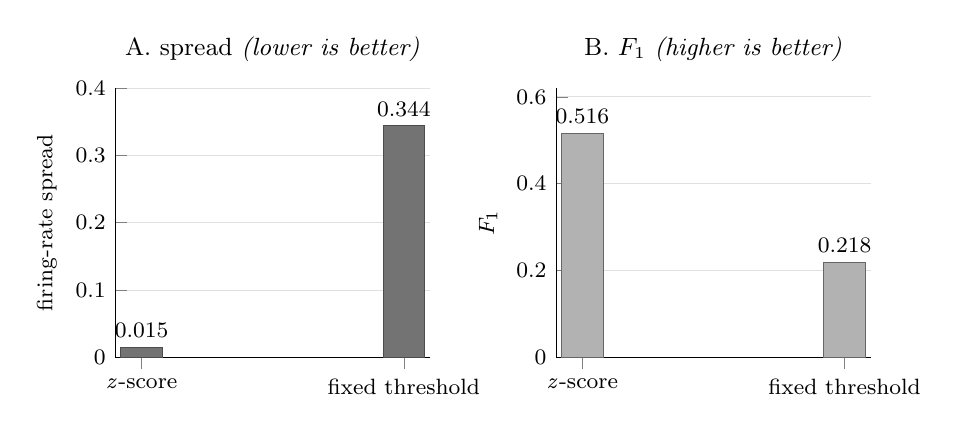
\begin{tikzpicture}
\begin{axis}[
  name=esq, width=0.46\textwidth, height=5.0cm, ybar, bar width=15pt,
  ymin=0, ymax=0.40, symbolic x coords={zscore, fixo}, xtick=data,
  xticklabels={\emph{z}-score, fixed threshold}, ylabel={firing-rate spread},
  nodes near coords, point meta=explicit symbolic,
  every node near coord/.append style={font=\footnotesize},
  title={\small A. spread \emph{(lower is better)}},
  tick label style={font=\footnotesize}, label style={font=\footnotesize},
  ymajorgrids, grid style={black!12}, axis lines*=left,
]
\addplot[fill=black!55, draw=black!70] coordinates {(zscore,0.015) [0.015] (fixo,0.344) [0.344]};
\end{axis}
\begin{axis}[
  name=dir, at={(esq.right of origin)}, anchor=left of origin, xshift=1.6cm,
  width=0.46\textwidth, height=5.0cm, ybar, bar width=15pt,
  ymin=0, ymax=0.62, symbolic x coords={zscore, fixo}, xtick=data,
  xticklabels={\emph{z}-score, fixed threshold}, ylabel={$F_1$},
  nodes near coords, point meta=explicit symbolic,
  every node near coord/.append style={font=\footnotesize},
  title={\small B. $F_1$ \emph{(higher is better)}},
  tick label style={font=\footnotesize}, label style={font=\footnotesize},
  ymajorgrids, grid style={black!12}, axis lines*=left,
]
\addplot[fill=black!30, draw=black!60] coordinates {(zscore,0.516) [0.516] (fixo,0.218) [0.218]};
\end{axis}
\end{tikzpicture}
\caption[The two measures of the first question]{The two measures, side by side. In A, the
difference between the maximum and the minimum rate across the fifteen companies; the fixed
threshold flags $0.9\%$ of the days in the calmest company and $35.3\%$ in the most volatile, while
the \emph{z}-score stays between $1.6\%$ and $3.1\%$ in all of them. In B, the performance against
the approximate label.}
\label{fig:av_amplitude}
\end{figure}

The firing-rate spread is $0.015$ for the \emph{z}-score and $0.344$ for the fixed threshold, a
difference of more than twenty times. Against the approximate label, the \emph{z}-score obtains
$F_1 = 0.516$ and the fixed threshold $0.218$.

The comparison involves an asymmetry of treatment. The window of the \emph{z}-score is varied
later in this section, whereas the three per cent threshold of the fixed rule is the conventional
value and was not optimised. What the comparison establishes with confidence is not that no fixed
threshold would obtain a better result, but that a fixed threshold measures a quantity different
from the one intended, because the same percentage corresponds to distinct rarities in distinct
companies. This argument does not depend on the value chosen.

\subsection{What the principal measure does not exclude}

The firing-rate spread has zero as its optimum, and that optimum is attainable by a method with no
information at all. A detector that flagged in each company a fixed fraction of days chosen at
random would show a practically null spread, beating the \emph{z}-score precisely on the measure
this section elects as principal. The claim follows from the construction of the method and
requires no execution.

The consequence is not that the measure is invalid, but that it must be read together with the
second, and that is why there are two. The spread excludes the fixed threshold, which fires as a
function of the volatility of the company and not of the rarity of the day. $F_1$ excludes random
firing, which sits at the level of chance against any label. Neither measure is sufficient on its
own, and only the rolling rule satisfies both.


An asymmetry in the standard of evidence applied throughout the chapter should also be recorded.
The values of this section and of the next are points, without confidence intervals, whereas those
of Section~\ref{sec:av_qi3}, where the result that contradicts the initial hypothesis resides, come
with resampling by groups. The partial justification lies in the order of magnitude of the
differences observed here, which no plausible resampling would reverse. The justification is not
complete, since days of the same company are also not independent observations in this case, for
the same reason of volatility clustering invoked later on.

\subsection{Comparison with learned detectors}

The most demanding comparison sets the statistical rule against machine learning methods designed
to detect anomalies. Two were evaluated, over the same information and under the same discipline of
not using information posterior to the day assessed: \emph{Isolation Forest}
\autocite{liu2008isolation} and the \emph{Local Outlier Factor} \autocite{breunig2000lof}. Both ran
in a single configuration, without a hyperparameter search, which limits the reach of their defeat
for the same reason invoked later for the tree model. What is established is that these detectors,
parameterised in this way and over these inputs, do not beat the rule; not that no parameterisation
would. Figure~\ref{fig:av_detetores} presents the result.

\begin{figure}[ht]
\centering
\begin{tikzpicture}
\begin{axis}[
  ig axis,
  width=0.78\textwidth, height=6.0cm,
  xmin=0, xmax=0.50, ymin=0, ymax=1.05,
  xtick={0,0.1,0.2,0.3,0.4,0.5},
  xticklabels={{0.0},{0.1},{0.2},{0.3},{0.4},{0.5}},
  ytick={0,0.2,0.4,0.6,0.8,1.0},
  yticklabels={{0.0},{0.2},{0.4},{0.6},{0.8},{1.0}},
  xlabel={precision}, ylabel={recall},
  xmajorgrids, ymajorgrids,
]
\addplot[ig current mark] coordinates {(0.407,0.761)};
\addplot[only marks, mark=triangle*, mark size=3.2pt, draw=igInk, fill=white]
  coordinates {(0.158,0.913)};
\addplot[only marks, mark=diamond*, mark size=3.2pt, draw=igInk, fill=igMist]
  coordinates {(0.163,0.989)};
\node[font=\scriptsize, align=right, anchor=south east, text=igGreenDark]
  at (axis cs:0.407,0.761) {\emph{z}-score\\$F_1=0.530$};
\node[font=\scriptsize, align=right, anchor=north east, text=igInk]
  at (axis cs:0.158,0.913) {Isolation Forest\\$F_1=0.269$};
\node[font=\scriptsize, align=left, anchor=north west, text=igInk]
  at (axis cs:0.163,0.989) {Local Outlier Factor\\$F_1=0.280$};
\end{axis}
\end{tikzpicture}
\caption[The transparent rule against two learned detectors]{The three detectors over the same data
and under the same protocol, restricted to the region all three can score. The two learned methods
occupy the region of near-total recall and low precision; the rule trades some recall for
precision. The $F_1$ beside each point summarises that trade-off. The firing-rate spread follows
the same pattern, at $0.017$ for the rule against $0.140$ and $0.183$ for the learned
detectors.}
\label{fig:av_detetores}
\end{figure}

The transparent rule beats both methods, with almost twice the $F_1$ and with substantially better
consistency across companies. This is the first of three cases, throughout the chapter, in which a
more sophisticated technique is compared under equivalent conditions with a simpler one and does
not obtain a better result. The choice of the simple method thus becomes justified by measurement
and not by preference.

The explanation does not lie in the quality of the methods. Both determine what is unusual from
the geometry of the data, by opposite routes. \emph{Isolation Forest} identifies the rare point by
how easily successive random cuts separate it from the rest \autocite{liu2008isolation}. The
\emph{Local Outlier Factor} compares the density in the neighbourhood of each point with that of
the points surrounding it \autocite{breunig2000lof}.

These are non-parametric methods, outside the statistical family that
\textcite{chandola2009anomaly} characterises by the modelling of the distribution of normal data,
and they were designed for sets with many interacting variables. The problem treated here has
another form: one series of returns per company, whose relevant structure is temporal. Volatility
clustering, formalised by \gls{ARCH} and \gls{GARCH} models \autocite{engle1982arch,
bollerslev1986garch}, moves over time the threshold of what constitutes an unusual day; a rolling
window follows that movement by construction, whereas a detector fitted to the complete set has to
infer it.

A note on the compatibility between the values: the \emph{z}-score appears with $F_1 = 0.530$ in
this comparison and with $0.516$ in the previous one. The two values measure the same detector
under distinct protocols. The second covers all the days assessed, while the first is restricted to
the region all three detectors can score, the only one in which the comparison between them is
fair. The spread follows the same rule, being $0.017$ under this protocol and $0.015$ under the
previous one.

\subsection{Two comparisons that do not confirm the deployed choices}

Two additional experiments were designed to justify options taken, and neither of them confirmed
them. Both are reported as they came out.

The first concerns the volatility estimator. The alternative to giving the same weight to the
twenty days of the window consists in giving greater weight to the recent days, through an
exponentially weighted average. Figure~\ref{fig:av_ewma} presents the result.

\begin{figure}[ht]
\centering
\begin{tikzpicture}
\begin{axis}[
  ig axis, ig legend,
  width=0.78\textwidth, height=4.8cm,
  xmin=0, xmax=1.0,
  symbolic y coords={f,c,p}, ytick={f,c,p},
  enlarge y limits=0.28,
  yticklabels={$F_1$, recall, precision},
  xlabel={metric value},
  xtick={0,0.2,0.4,0.6,0.8,1.0},
  xticklabels={{0.0},{0.2},{0.4},{0.6},{0.8},{1.0}},
  xmajorgrids,
  legend style={at={(0.5,1.04)}, anchor=south, legend columns=2},
]
\addplot[ig connector, forget plot] coordinates {(0.381,p) (0.568,p)};
\addplot[ig connector, forget plot] coordinates {(0.800,c) (0.800,c)};
\addplot[ig connector, forget plot] coordinates {(0.516,f) (0.664,f)};
\addplot[ig current mark] coordinates {(0.381,p) (0.800,c) (0.516,f)};
\addlegendentry{equal weights (deployed)}
\addplot[ig alternative mark] coordinates {(0.568,p) (0.800,c) (0.664,f)};
\addlegendentry{exponential decay}
\node[font=\scriptsize, anchor=south east, text=igGreenDark] at (axis cs:0.381,p) {0.381};
\node[font=\scriptsize, anchor=south west, text=igInk] at (axis cs:0.568,p) {0.568};
\node[font=\scriptsize, anchor=south, text=igInk] at (axis cs:0.800,c) {0.800 in both};
\node[font=\scriptsize, anchor=south east, text=igGreenDark] at (axis cs:0.516,f) {0.516};
\node[font=\scriptsize, anchor=south west, text=igInk] at (axis cs:0.664,f) {0.664};
\end{axis}
\end{tikzpicture}
\caption[Two volatility estimators under the same protocol]{The two estimators, with the same
recall; each segment links the deployed result to the alternative on the same measure. The
exponentially weighted alternative removes almost half the false alarms, raising precision from
$0.381$ to $0.568$, and is even more consistent across companies, with a spread of $0.012$ against
$0.015$. The system keeps the estimator that obtained the inferior result, for the reason set out
in the text.}
\label{fig:av_ewma}
\end{figure}

With identical recall, the alternative obtains $F_1 = 0.664$ against $0.516$ for the deployed
estimator. The mechanism is understandable. Large movements occur in clusters. A twenty-day average
with equal weights dilutes a shock over twenty observations and keeps flagging the following days
for weeks; an average that favours the recent past absorbs it immediately.

The system keeps the estimator that obtained the inferior result. The reason is the one that runs
through the work: the mean and the standard deviation of the last twenty days can be explained in
two sentences to any reader, and exponentially decaying weights cannot. In a tool whose central
argument is explainability, a gain in precision obtained at the cost of the explanation is not
unequivocally a gain. It is recorded, however, as a choice and not as a result: the alternative is
measured, the gain is quantified, and adopting it would be a small change should explainability
cease to be the dominant constraint.

The second experiment concerns the size of the window, and Figure~\ref{fig:av_janela} presents
it.

\begin{figure}[ht]
\centering
\begin{tikzpicture}
\begin{axis}[
  width=0.72\textwidth, height=5.0cm,
  xlabel={estimation window (trading days)},
  ylabel={$F_1$ against the approximate label},
  xmin=4, xmax=72, ymin=0.30, ymax=0.76,
  xtick={10,20,60}, ytick={0.4,0.5,0.6,0.7},
  yticklabels={{0.4},{0.5},{0.6},{0.7}},
  tick label style={font=\footnotesize}, label style={font=\footnotesize},
  ymajorgrids, grid style={black!12}, axis lines*=left,
  nodes near coords, point meta=explicit symbolic,
  every node near coord/.append style={font=\scriptsize, anchor=north west},
]
\addplot[black!70, thick, mark=*, mark size=2pt]
  coordinates {(10,0.385) [0.385] (20,0.516) [0.516] (60,0.678) [0.678]};
\addplot[ig current mark, nodes near coords={}] coordinates {(20,0.516)};
\draw[dashed, igGreenDark] (axis cs:20,0.30) -- (axis cs:20,0.505);
\node[text=igGreenDark, font=\scriptsize, anchor=south west] at (axis cs:21,0.31) {deployed window};
\end{axis}
\end{tikzpicture}
\caption[Ablation on the size of the window]{Performance against the approximate label for three
window sizes. The value grows monotonically with the size of the window, and the deployed window is
not the one that obtains the best result. The text sets out the two reasons why the longer window
was not adopted, the second being a reservation about the validity of this measurement itself.}
\label{fig:av_janela}
\end{figure}

A sixty-day window obtains $F_1 = 0.678$ against the $0.516$ of the twenty-day window. Two reasons
justify keeping the shorter window. The first is responsiveness: a sixty-day window takes three
months to react to a change of regime, and a company moving from calm to volatile would continue to
be judged by the previous norm.

The second concerns the validity of this particular measurement. The label is built from the
percentile of movement of the company itself, and is therefore relative to volatility; a longer
window produces a less adaptive norm, which flags the extreme tail more often, which is precisely
what this label rewards. Circularity exists, and it favours the long window by construction. This
is why the principal argument of this section is the consistency of the firing rate, which uses no
labels. The formulation that survives is that the twenty-day window was chosen for responsiveness,
and that the only measurement available on this point does not support it.

\subsection{Limits of the conclusion}

The label is approximate and relative to volatility, which is why the argument that carries weight
is the one about consistency, which does not depend on it. The fifteen companies are all
large-capitalisation and were selected in 2026, with the evaluation running over the past: they
survived by construction, and none of them was delisted, absorbed or dropped from the list. What is
measured is the behaviour of the method in companies that persisted, and not in the population from
which they were drawn. The comparison covers
this set and this period only, and nothing in it allows the result in another market or another
decade to be anticipated.

\section{Precedent retrieval}
\label{sec:av_qi2}

The second case study answers \gls{QI}2: retrieval by meaning finds past news from another company
in the same sector better than trivial alternatives. The answer is affirmative in the five sectors
assessed, and the per-sector formulation is necessary, since the aggregate value is misleading in
both directions.

\subsection{Procedimento}

Evaluating retrieval systems faces the absence of a list of correct answers, since no set of pairs
of news items is annotated as related. A verifiable approximation is therefore used: a retrieved
news item is considered relevant if it belongs to the same sector as the query news item. The
approximation is imperfect, because two news items from the same sector may deal with distinct
subjects, but it is objective and was fixed before the results were observed.

A further constraint is imposed that makes the task harder: the retrieved news item must belong to
a different company. Without it, the system would perform well by returning news from the company
itself, which almost always belongs to the same sector by construction. The corpus contains
$3{,}714$ news items distributed across five sectors, collected over twenty-seven days, and the
measurement uses five hundred queries per repetition across five repetitions with distinct seeds.
The span of the corpus delimits what the measurement establishes: twenty-seven days do not support
claims about temporal generalisation. The protocol does not require the candidate to be prior to
the query, and only $31.1\%$ of the neighbours are. The check under the causal constraint was made
in aggregate over the historical corpus, where the margin over chance holds, and not per sector.

\subsection{Result}

Figure~\ref{fig:av_recuperacao} presents the method used, a larger variant and the trivial
alternatives.

\begin{figure}[ht]
\centering
\begin{tikzpicture}
\begin{axis}[
  ig axis,
  xbar, width=0.70\textwidth, height=6.6cm, bar width=9pt,
  xmin=0, xmax=0.66, enlarge y limits=0.10,
  symbolic y coords={rec, aleat, maior, lex, fin, mini, mpnet},
  ytick={rec, aleat, maior, lex, fin, mini, mpnet},
  yticklabels={Most recent, Random choice, Always the largest sector, Shared words,
               Finance encoder, Embeddings (MiniLM), Embeddings (MPNet)},
  ig values,
  xlabel={precision@5},
  xmajorgrids,
]
\addplot[bar shift=0pt, ig alternative bar] coordinates {
  (0.126,rec) [0.126] (0.240,aleat) [0.240] (0.346,lex) [0.346]
  (0.420,fin) [0.420]};
\addplot[bar shift=0pt, ig reference bar] coordinates {(0.467,maior) [0.467]};
\addplot[bar shift=0pt, ig current bar] coordinates {(0.514,mini) [0.514]};
\addplot[bar shift=0pt, ig competitor bar] coordinates {(0.538,mpnet) [0.538]};
\end{axis}
\end{tikzpicture}
\caption[Retrieval: the method against six alternatives]{Precision@5 of the deployed MiniLM, in
solid green, against six alternatives. The green outline identifies the larger MPNet variant; the
grey bars bring together two baselines, a lexical one and an encoder specific to the financial
domain. The dashed alternative of always returning news from the largest sector obtains $0.467$
without any model, a value discussed in the text and one that requires the aggregate to be read
with reservation.}
\label{fig:av_recuperacao}
\end{figure}

Random choice is right in $24.0\%$ of cases, and that is the reference value, and not zero, since
the sectors are finite in number and of distinct sizes. Search by words in common raises the result
to $34.6\%$, and comparison by meaning to $51.4\%$.

The lexical baseline is the simplest form of that family: word counts projected by hashing and
compared by cosine, without weighting by the rarity of terms, without frequency saturation and
without normalisation by the length of the text. It belongs to the tradition that runs from the
vector space model \autocite{salton1975vsm} to probabilistic ranking functions such as BM25
\autocite{robertson2009bm25}, sitting on the first step of that family. The seventeen percentage
points that the sentence representation \autocite{reimers2019sbert} adds therefore measure the
distance to an elementary starting point and not the distance to a tuned lexical system. The
comparison with a well-parameterised ranking function is work still to be done, and it is the one
that would make this conclusion stronger.

The encoder specific to the financial domain obtains $0.420$, the lowest value of all the models
assessed. The model assessed is the public checkpoint \texttt{ProsusAI/finbert}, identified in this
way because it is the exact artefact the measurement bears on; it belongs to the family of
financial encoders of which \textcite{liu2020finbert} and \textcite{huang2023finbert} are the
versions documented in peer-reviewed publications. It was used with the mean of its vectors as the
sentence representation, which is the way to apply it without further training. It is an encoder
tuned for sentiment classification and not for positioning sentences in a space where distance
means similarity, and it is precisely that training objective that Sentence-BERT adds
\autocite{reimers2019sbert}. The measurement establishes that this domain model, used in this way,
obtains a result inferior to a generic model trained for similarity; it does not establish that
domain knowledge is irrelevant to the task.

\subsection{The trivial alternative the aggregate hides}

The corpus is not balanced: $1{,}736$ of the $3{,}714$ news items, almost half, belong to the
technology sector. There is therefore a strategy that dispenses with any model and does not even
look at the query, consisting in invariably returning five technology news items. It is right on
every technology query and on none of the others, so its precision equals exactly the fraction of
queries that are about technology, $0.467$. Measured against this alternative, and not against
uniform chance, the margin of the method falls from $+0.274$ to $+0.047$, and the lexical baseline
of $0.346$ comes to sit below the reference value.

The aggregate value is, however, the misleading element, and not the method. The trivial strategy
obtains $1.000$ on technology queries and $0.000$ on all the others, returning semiconductor news to
someone querying about an oil company. What it exploits is not a property of the problem, but the
composition of this corpus.

The comparison that survives this objection is the one carried out within each sector, where the
trivial strategy has nothing to lean on. Panel A of Figure~\ref{fig:av_setor_causal} presents
it.

\begin{figure}[ht]
\centering

\includegraphics[width=0.96\textwidth]{figures/eval_retrieval_sector_causal.pdf}
\caption[Retrieval by sector and under the temporal constraint]{In A, precision@5 and the
corresponding chance value within each sector: the method sits above its reference value in all
five. In B, the symmetric protocol of the scale test and the causal protocol that reproduces the
constraint of production, each beside its reference value. Precision falls from $0.595$ to $0.513$
and the chance value from $0.333$ to $0.259$, so the margin varies only from $+0.262$ to
$+0.254$.}
\label{fig:av_setor_causal}
\end{figure}

The chance value is $0.429$ in technology and stands around $0.072$ in each of the four remaining
sectors. The method obtains $0.712$ in technology, $0.448$ in energy, $0.419$ in health, $0.272$ in
banking and $0.171$ in consumer. Where the aggregate is dominated, the method adds $0.283$; where
the corpus is sparse, it obtains several times the reference value. The aggregate underestimates
the method and overestimates the trivial alternative for the same reason, which is that almost half
the queries come from the single sector where the reference value was already high. The claim the
work supports is therefore the narrowest one: semantic retrieval beats the base rate within each of
the five sectors, and the aggregate value is not the appropriate way of stating it.

The larger variant obtains $0.538 \pm 0.011$ against $0.514 \pm 0.015$ for the one used, over five
seeds; the difference is small relative to the dispersion and no significance test was carried out.
Two more recent encoders obtain $0.504$ and $0.513$, indistinguishable from the deployed one. The
adoption of the smaller model in production followed from computational cost and not from an
advantage in quality, and is an explicit trade whose price in precision is quantified. The
apparently most reasonable alternative, which consists in presenting the most recent news, obtains
$0.126$, the lowest value of all, which is consistent with there being no reason for the most
recent news item about another company to be related to the news item under analysis.

\subsection{Behaviour at scale and under the production constraint}

The previous evaluation bears on a recent corpus of limited size. To verify that the result does
not depend on that corpus, the same measurement was repeated over the complete historical set, with
approximately eighty thousand news items from six years. Under this symmetric protocol, which still
admits candidates posterior to the query, precision@5 rises to $0.595$. The rise should not,
however, be read in full as a gain: the chance value rises likewise, from $0.240$ to $0.333$,
because the composition by sector is different. Measured against the respective reference value,
the margin is $+0.274$ in the first case and $+0.262$ in the second. The result establishes that the
method does not degrade when the corpus goes from recent and short to six years, and not that it
improves with more data.

The previous protocol grants a freedom the system in production does not have. The only constraint
imposed is that the candidate belong to another company, which allows it to be posterior to the
query, and that case is common: in the recent corpus, $38.7\%$ of the neighbours returned are dated
after the query and another $30.2\%$ are from the same day. The deployed system does not have that
freedom, since the precedent base only receives a case eight days after it is observed, as
Section~\ref{sec:sis_base} describes.

This is not use of future information in the usual sense. The criterion for a hit is membership of
the same sector, and the sector of a news item does not vary with time, so the temporal direction
cannot inflate precision. What is at stake is the correspondence between the value reported and the
task the research question describes, which speaks of past news. The measurement repeats the
protocol adding to the mask the condition that the candidate be strictly prior to the query, and
reproduces the symmetric value in the same run so that the comparison is paired. None of the
$2{,}500$ queries was left without sufficient past. The result appears in panel B of
Figure~\ref{fig:av_setor_causal}: precision falls by $0.082$, the reference value falls by almost
as much, and the margin varies by $0.008$. The method keeps practically all of its advantage when
forced to operate as it operates in production.

This is the third occasion in the chapter on which reading a precision without its corresponding
reference value would lead to the wrong conclusion. It happened in the move from the recent corpus
to the complete one, it happens with the precision within the budget treated in
Section~\ref{sec:av_qi3}, and it happens here. Precision is a quantity with no meaning of its own,
which it acquires only alongside the alternative that has no information.

\subsection{Limites da conclusão}

Membership of the same sector is not equivalent to a relation between news items; it is an
approximation built because it is verifiable and not because it corresponds exactly to the property
intended.

The second observation has consequences for the product: retrieval captures topic and not
direction. Two news items can deal with the same subject and the price move in opposite directions,
which is what happened in the example presented in Chapter~\ref{cap:sistema}.
Figure~\ref{fig:av_direcao} quantifies it.

\begin{figure}[ht]
\centering
\begin{tikzpicture}
\begin{axis}[
  ig axis, ig legend,
  width=0.72\textwidth, height=3.2cm,
  xmin=0, xmax=1, ymin=0.6, ymax=1.4,
  ytick={1}, yticklabels={same direction},
  xlabel={direction agreement between query and precedent},
  xtick={0,0.25,0.50,0.75,1.0}, xticklabels={{0.00},{0.25},{0.50},{0.75},{1.00}},
  xmajorgrids,
  legend style={at={(0.5,1.05)}, anchor=south, legend columns=2},
]
\addplot[ig connector, forget plot] coordinates {(0.688,1) (0.708,1)};
\addplot[ig alternative mark] coordinates {(0.688,1)};
\addlegendentry{random pairing}
\addplot[ig current mark] coordinates {(0.708,1)};
\addlegendentry{retrieved cases}
\node[font=\scriptsize, anchor=south east, text=igInk] at (axis cs:0.688,1) {0.688};
\node[font=\scriptsize, anchor=south west, text=igGreenDark] at (axis cs:0.708,1) {0.708};
\end{axis}
\end{tikzpicture}
\caption[Topic and direction are not the same property]{Fraction of retrieved cases whose price
moved in the same direction as that of the query news item, against the value obtained by random
pairing under the same constraints, on a full scale between zero and one. The difference is
$0.020$. The system therefore presents the cases individually, and the text of the alert states
that the similarity is one of topic.}
\label{fig:av_direcao}
\end{figure}

The direction agreement between the query news item and the retrieved cases stands at $0.708$
against a chance value of $0.688$. It is for this reason that the system presents the cases one by
one and never summarises them into an average, which would be read as a forecast, and that the text
of the alert explicitly states that these are cases similar in topic.

\section{News triage}
\label{sec:av_qi3}

The third case study answers \gls{QI}3: a trained model prioritises news better than a baseline
built only on volatility. The answer is negative, and it is the result with the greatest
informative value in the work.

\subsection{Procedimento}

O conjunto de dados contém $79{,}753$ exemplos entre 2018 e 2023, cada um correspondente a uma notícia
com o contexto de mercado do dia e o rótulo definido na Secção~\ref{sec:met_triagem}. A divisão é
cronológica com embargo, e a prevalência de casos positivos no bloco de teste é de $0.378$. A
métrica principal é a \gls{PRAUC}, adequada quando as duas classes estão desequilibradas.

Para efeitos práticos, uma diferença de \gls{PRAUC} inferior a $0.02$ é tratada como
indistinguível, mesmo quando o intervalo emparelhado exclui zero. O limite é uma escolha do autor,
declarada antes dos resultados, o que obriga à sua aplicação nos dois sentidos.

Dois cuidados de montagem asseguram que a comparação não favorece a conclusão obtida. O primeiro é a
inclusão de um conjunto de árvores treinado por reforço do gradiente \autocite{friedman2001gbm}, o
mais expressivo dos modelos comparados, por captar interações e efeitos não lineares que a regressão
logística não capta por construção. Este modelo foi executado com os parâmetros por defeito da
biblioteca, sem procura de hiperparâmetros, o que limita o alcance da sua derrota: estabelece que o
texto não produz vantagem nesta montagem, e não que a não produziria num modelo não linear afinado.
O segundo cuidado é a conversão de todas as pontuações em probabilidades por calibração \emph{a
posteriori} sobre um bloco de validação reservado \autocite{niculescu2005calibration}, sem a qual a
comparação pelo índice de Brier não seria válida entre modelos.

Uma entrada não está disponível no mesmo referencial em produção. O retorno do próprio dia
corresponde, no conjunto histórico, ao movimento completo do dia da notícia, ao passo que em produção
a notícia é pontuada antes de esse dia encerrar. O resultado apresentado avalia por isso o modelo com
a variável diária completa e não demonstra paridade com a pontuação intradiária. A direção da assimetria é conhecida. A entrada em causa pertence ao bloco de contexto, presente
nos modelos de resultado inferior. A linha de base vencedora usa uma só entrada: a volatilidade
dos vinte dias anteriores, fechada na véspera. O referencial mais generoso
encontra-se do lado dos modelos que a comparação não favorece, e a sua correção só poderia tornar o
resultado negativo mais forte.

\subsection{Resultado}

A Figura~\ref{fig:av_triagem} apresenta os cinco modelos e a referência sem informação comparados. As curvas completas, de que estes valores são a área, constam dos artefactos identificados no
Apêndice~\ref{ap:reprodutibilidade}. Nelas a curva da volatilidade situa-se acima das restantes em
quase toda a extensão do eixo, o que estabelece que a diferença não é artefacto do valor agregado.

\begin{figure}[ht]
\centering
\begin{tikzpicture}
\begin{axis}[
  ig axis,
  width=0.72\textwidth, height=6.4cm,
  xmin=0, xmax=0.66, enlarge y limits=0.12,
  symbolic y coords={texto, gbm, ctxtexto, ctx, vol},
  ytick={texto, gbm, ctxtexto, ctx, vol},
  yticklabels={Headline text only, Trees with context and text,
               Context and text, Market context only, Volatility only},
  xlabel={\gls{PRAUC} on the test block},
  xmajorgrids,
]
\addplot[ig interval] coordinates {(0.406,texto) (0.474,texto)};
\addplot[ig interval] coordinates {(0.427,gbm) (0.517,gbm)};
\addplot[ig interval] coordinates {(0.453,ctxtexto) (0.540,ctxtexto)};
\addplot[ig interval] coordinates {(0.487,ctx) (0.592,ctx)};
\addplot[ig interval] coordinates {(0.492,vol) (0.597,vol)};
\addplot[only marks, mark=|, mark size=3.4pt, draw=igSlate] coordinates {
  (0.406,texto) (0.474,texto) (0.427,gbm) (0.517,gbm)
  (0.453,ctxtexto) (0.540,ctxtexto) (0.487,ctx) (0.592,ctx)};
\addplot[only marks, mark=|, mark size=3.4pt, draw=igSlate] coordinates {
  (0.492,vol) (0.597,vol)};
\addplot[ig alternative mark] coordinates {
  (0.439,texto) (0.469,gbm) (0.496,ctxtexto) (0.542,vol)};
\addplot[ig current mark] coordinates {(0.538,ctx)};
\draw[draw=igInk, densely dashed, line width=1pt] (axis cs:0.378,texto) -- (axis cs:0.378,vol);
\node[font=\scriptsize, anchor=south west, text=igInk] at (axis cs:0.378,vol)
  {prevalence 0.378};
\end{axis}
\end{tikzpicture}
\caption[Triagem: pontos e intervalos sobre o mesmo bloco de teste]{Área sob a curva de precisão e
cobertura de cinco modelos, com intervalos marginais a noventa e cinco por cento obtidos por
reamostragem dos $1{,}951$ grupos. A linha tracejada assinala a prevalência do bloco de teste, que é o valor
obtido por um modelo que atribua a mesma probabilidade a todos os exemplos. Os valores são pontos, e
os intervalos são amplos e sobrepõem-se: $[0.492;\,0.597]$ para a volatilidade, $[0.487;\,0.592]$ para o
contexto e $[0.453;\,0.540]$ para o contexto com texto. A comparação que a subsecção seguinte
sustenta é a diferença emparelhada entre modelos sobre as mesmas reamostragens, e não a distância
entre dois pontos.}
\label{fig:av_triagem}
\end{figure}


O valor mais elevado pertence ao modelo mais simples de todos, o que utiliza apenas a volatilidade
recente. Acrescentar-lhe o restante contexto não altera o resultado de forma distinguível, com
$0.538$ contra $0.542$; acrescentar o texto do título deteriora-o de forma distinguível, com
$0.496$. O índice de Brier acompanha a mesma ordenação, com $0.218$ para o modelo de
volatilidade contra $0.229$ para o modelo com texto e $0.622$ para o modelo que anuncia sempre a
unidade. A hipótese inicial, segundo a qual o texto da notícia traria informação ausente dos preços,
não é confirmada sobre este corpus.

\subsection{Três verificações à montagem experimental}

O resultado negativo foi submetido a três verificações destinadas a determinar se decorre da montagem
experimental.

A primeira respeita ao ajuste do modelo de texto. A comparação foi repetida concedendo ao texto as
melhores condições disponíveis, com regularização afinada, redução do bloco de texto a trinta e duas
dimensões e um modelo de linguagem especializado em finanças. O melhor resultado do texto sobe para
$0.533$ e permanece abaixo dos $0.542$ da volatilidade.

A segunda respeita ao ruído de amostragem. O bloco de teste foi reamostrado mil vezes por grupos
constituídos pela empresa e pelo dia, uma vez que notícias do mesmo dia sobre a mesma empresa
partilham o rótulo e não constituem observações independentes. A diferença entre a volatilidade e a
variante com texto é de $+0.048$, com intervalo entre $+0.032$ e $+0.066$, que exclui zero e
supera o limite prático de $0.02$. É a única comparação desta secção que o supera.

O alcance deste
intervalo é, contudo, limitado: a reamostragem realiza-se dentro de
um único bloco de teste, com duzentos e vinte e um dias de negociação, pelo que mede o ruído de
amostragem nesse período e nada estabelece sobre a estabilidade entre períodos. A distinção não é
teórica neste trabalho, dado que a Secção~\ref{sec:av_producao} reporta um deslocamento significativo
na distribuição da entrada principal. Uma origem rolante com três ou quatro cortes sucessivos
responderia à pergunta mais larga, e não foi realizada.

A terceira respeita à definição do rótulo, que utiliza um limiar de dois por cento e um horizonte de
três dias, ambos escolhidos pelo autor. A comparação foi repetida para nove combinações de limiar e
horizonte, e a Figura~\ref{fig:av_rotulos} apresenta o resultado.

\begin{figure}[ht]
\centering
\begin{tikzpicture}
\begin{groupplot}[
  group style={group size=3 by 1, horizontal sep=0.55cm,
    ylabels at=edge left, yticklabels at=edge left},
  ig axis, ig legend,
  width=0.29\textwidth, height=4.8cm,
  xmin=0.5, xmax=5.5, ymin=0, ymax=0.82,
  xtick={1,3,5}, xlabel={horizon (days)},
  ytick={0,0.2,0.4,0.6,0.8},
  yticklabels={{0.0},{0.2},{0.4},{0.6},{0.8}},
  ymajorgrids,
  legend columns=3,
]
\nextgroupplot[title={threshold 1.5\%}, ylabel={\gls{PRAUC}}, legend to name=leg:rotulos]
\addplot[ig comparison line] coordinates {(1,0.449) (3,0.613) (5,0.716)};
\addlegendentry{volatility only}
\addplot[ig alternative line] coordinates {(1,0.420) (3,0.572) (5,0.689)};
\addlegendentry{context and text}
\addplot[ig reference line] coordinates {(1,0.277) (3,0.483) (5,0.597)};
\addlegendentry{prevalence}

\nextgroupplot[title={threshold 2\%}]
\path[fill=igGreenLight] (axis cs:2.55,0) rectangle (axis cs:3.45,0.82);
\addplot[ig comparison line] coordinates {(1,0.334) (3,0.542) (5,0.620)};
\addplot[ig alternative line] coordinates {(1,0.294) (3,0.496) (5,0.590)};
\addplot[ig reference line] coordinates {(1,0.183) (3,0.378) (5,0.487)};
\node[font=\scriptsize, text=igGreenDark, anchor=south] at (axis cs:3,0.72) {cell reported};

\nextgroupplot[title={threshold 3\%}]
\addplot[ig comparison line] coordinates {(1,0.228) (3,0.402) (5,0.489)};
\addplot[ig alternative line] coordinates {(1,0.174) (3,0.369) (5,0.461)};
\addplot[ig reference line] coordinates {(1,0.082) (3,0.232) (5,0.324)};
\end{groupplot}
\end{tikzpicture}
\par\smallskip
\pgfplotslegendfromname{leg:rotulos}
\caption[O resultado sob nove definições alternativas de rótulo]{Desempenho das duas famílias sob
os três horizontes, em três painéis correspondentes aos limiares, com a prevalência de cada célula
como referência. A faixa verde identifica a definição utilizada no restante capítulo. A
volatilidade iguala ou supera o modelo com texto nas nove combinações, com prevalências entre
$0.082$ e $0.597$.}
\label{fig:av_rotulos}
\end{figure}

O resultado negativo resiste às três verificações. A volatilidade iguala ou supera o modelo com texto
nas nove definições de rótulo, com prevalências entre $0.082$ e $0.597$, o que retira à escolha
concreta de limiar e horizonte o estatuto de ponto de ataque.

Uma quarta verificação incide sobre a composição dos blocos e conduz a uma conclusão que atua nos
dois sentidos. Os três blocos quase não partilham empresas. O bloco de treino decorre entre 2 de
janeiro de 2018 e 3 de março de 2022 e contém treze empresas; o bloco de teste decorre entre 2 de
fevereiro e 18 de dezembro de 2023 e contém nove. Cinco empresas do treino não figuram uma única vez
no teste, e uma empresa do teste, responsável por $17.1\%$ das suas linhas, nunca figura no treino.
Para as empresas presentes em ambos os lados, a taxa de positivos desloca-se de forma acentuada, e a
Apple passa de $0.448$ no treino para $0.183$ no teste. Estes valores leem-se diretamente das
colunas de identificação e de bloco do conjunto congelado e não exigem qualquer execução adicional.

Não se trata de utilização de informação futura nem de erro de divisão: o corte é realizado por dia,
e a proporção respeita a definida na Secção~\ref{sec:met_triagem}. É a composição do corpus que varia
com o tempo, pela mesma razão que torna o bloco de teste maior do que o de treino, uma vez que as
empresas sobre as quais se escreve em 2018 não são as mesmas de 2023.

A favor do resultado negativo pesa o seguinte. O sinal do modelo é essencialmente a identidade da
empresa, conforme a Secção~\ref{sec:av_ablacao} estabelece, e essa identidade é estimada sobre um
conjunto de empresas quase ausente do bloco onde é avaliada. A volatilidade dos vinte dias
anteriores, fechada na véspera, é comparável entre empresas e não depende da identidade de
nenhuma. Contra o
resultado, a comparação não separa a hipótese de o modelo ser pior da hipótese de a identidade não
transferir entre estes dois períodos, separação que exigiria uma divisão de composição constante. A
mesma constatação explica, sem recurso ao acaso, a prevalência de $47.0\%$ da validação contra
$37.8\%$ do teste, que correspondem a conjuntos de empresas distintos e não apenas a períodos
distintos.

\subsection{Utilidade sob a restrição de orçamento}

O produto apresenta no máximo cinco alertas por dia, pelo que a pergunta com significado operacional
é a de qual a fração de acertos entre as cinco notícias escolhidas em cada dia. A
Figura~\ref{fig:av_orcamento} isola duas referências que parecem equivalentes, mas não são.
O modelo e a alternativa baseada em volatilidade são comparados na
Figura~\ref{fig:av_pontaaponta}.

\begin{figure}[ht]
\centering
\begin{tikzpicture}
\begin{axis}[
  ig axis, xbar, width=0.68\textwidth, height=3.5cm, bar width=10pt,
  xmin=0, xmax=0.80, enlarge y limits=0.18,
  symbolic y coords={alfa, acaso},
  ytick={alfa, acaso},
  yticklabels={Alphabetical tie-break, Random choice},
  nodes near coords, nodes near coords align={horizontal}, point meta=explicit symbolic,
  every node near coord/.append style={font=\footnotesize},
  xlabel={precision within the five-alert daily budget},
  tick label style={font=\footnotesize}, label style={font=\footnotesize},
  xmajorgrids, grid style={black!12}, axis lines*=left,
]
\addplot[bar shift=0pt, ig alternative bar] coordinates {(0.163,alfa) [0.163]};
\addplot[bar shift=0pt, ig reference bar] coordinates {(0.379,acaso) [0.379]};
\end{axis}
\end{tikzpicture}
\caption[O desempate alfabético não é uma referência aleatória]{Duas formas de escolher as cinco
notícias do dia, sobre o mesmo bloco de teste. O desempate alfabético não mede escolha às cegas;
a escolha aleatória obtém $0.379 \pm 0.017$ sobre
quarenta sementes. As duas políticas escolhem conhecendo o dia completo, pelo que os valores são
limites superiores do que uma política em linha consegue obter.}
\label{fig:av_orcamento}
\end{figure}

A referência alfabética exige uma explicação: a designação original, «alertar sempre», induz em erro. O modelo que
alerta sempre atribui a mesma pontuação a todas as notícias, e quando todas empatam a métrica
seleciona pela ordem em que as linhas surgem no ficheiro, que está ordenado por data e por nome da
empresa. Esse valor de $0.163$ mede a escolha por ordem alfabética e não a escolha aleatória, e
todas as linhas que seleciona pertencem à empresa que ocupa a primeira posição no alfabeto. Comparado
com o valor de referência correto, o ganho do modelo é de $1.67$ vezes e não das quase quatro vezes
que a primeira leitura sugeriria. A lição é geral e aplica-se ao restante capítulo: verificar o que a
linha de base mede é tão necessário quanto verificar o que o modelo faz.

A comparação com a volatilidade, na Figura~\ref{fig:av_pontaaponta}, contém o resultado incómodo. Uma tabela de treze constantes,
correspondentes à volatilidade média de cada empresa, calculada exclusivamente sobre o bloco de
treino e sem leitura de um único título, obtém $0.662$ e supera o modelo treinado. A comparação
tem uma reserva que a torna menos limpa do que parece: $17.1\%$ das linhas do bloco de teste
pertencem a uma empresa ausente do treino e recebem a mediana global em vez de uma constante
própria. É, ainda assim, o terceiro caso do capítulo em que o método mais simples obtém melhor
resultado. O que a evidência sustenta é
que ordenar por volatilidade compensa, e não que aprender compense.

\subsection{Ablação das entradas do modelo}
\label{sec:av_ablacao}

O resultado anterior sugere que o modelo implantado reconhece a empresa e não a notícia. A
verificação dessa hipótese consiste em tentar reproduzi-lo com uma tabela de consulta que atribua a
cada empresa um único número fixado no bloco de treino, correspondente à fração das suas notícias que
se revelaram materiais. Essa tabela não observa o título, não observa o dia e devolve invariavelmente
o mesmo valor para a mesma empresa. A Figura~\ref{fig:av_ablacao} compara-a com o modelo implantado e
desmonta o modelo entrada a entrada, sob o protocolo congelado.

\begin{figure}[ht]
\centering
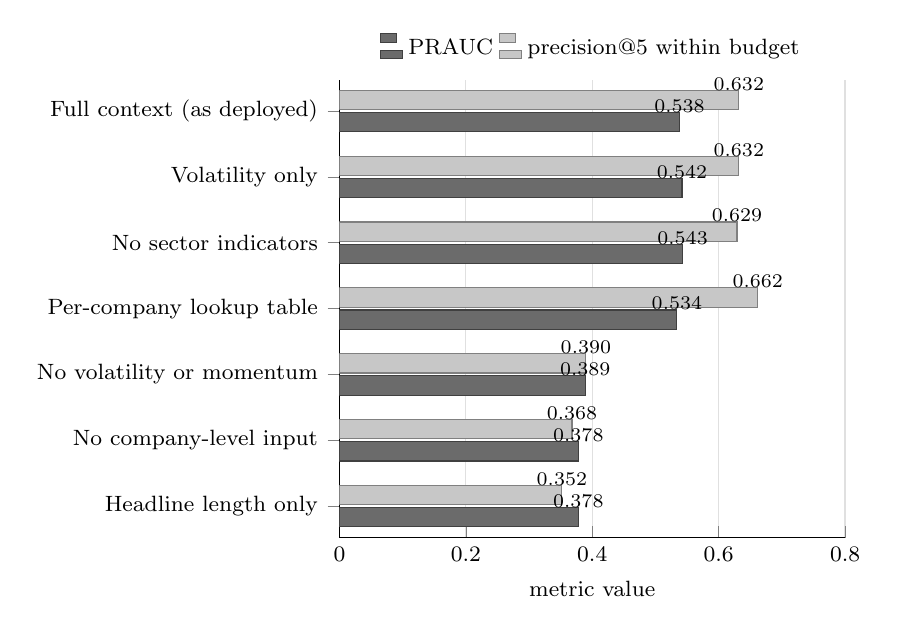
\begin{tikzpicture}
\begin{axis}[
  xbar=1pt, width=0.66\textwidth, height=7.4cm, bar width=7pt,
  xmin=0, xmax=0.80, enlarge y limits=0.08,
  symbolic y coords={comp, nada, semvol, tabela, semset, vol, ctx},
  ytick={comp, nada, semvol, tabela, semset, vol, ctx},
  yticklabels={Headline length only, No company-level input,
               No volatility or momentum, Per-company lookup table,
               No sector indicators, Volatility only,
               Full context (as deployed)},
  legend style={at={(0.5,1.02)}, anchor=south, legend columns=2, font=\footnotesize, draw=none},
  nodes near coords, nodes near coords align={horizontal}, point meta=explicit symbolic,
  every node near coord/.append style={font=\scriptsize},
  xlabel={metric value},
  tick label style={font=\footnotesize}, label style={font=\footnotesize},
  xmajorgrids, grid style={black!12}, axis lines*=left,
]
\addplot[fill=black!58, draw=black!75] coordinates {
  (0.378,comp) [0.378] (0.378,nada) [0.378] (0.389,semvol) [0.389] (0.534,tabela) [0.534]
  (0.543,semset) [0.543] (0.542,vol) [0.542] (0.538,ctx) [0.538]};
\addplot[fill=black!22, draw=black!50] coordinates {
  (0.352,comp) [0.352] (0.368,nada) [0.368] (0.390,semvol) [0.390] (0.662,tabela) [0.662]
  (0.629,semset) [0.629] (0.632,vol) [0.632] (0.632,ctx) [0.632]};
\legend{\gls{PRAUC}, precision@5 within budget}
\end{axis}
\end{tikzpicture}
\caption[O modelo comparado com subconjuntos das entradas]{Cada linha corresponde a uma variante
com um subconjunto das entradas ou a uma referência alternativa; as linhas não formam uma sequência
de remoções cumulativas. A linha decisiva é a da tabela de consulta, que não observa a notícia e
iguala o modelo implantado na primeira medida e o supera na segunda. As duas linhas inferiores, que
não dispõem de qualquer entrada de nível de empresa, situam-se exatamente na prevalência do bloco de
teste.}
\label{fig:av_ablacao}
\end{figure}

Três leituras resultam da figura, e nenhuma depende de interpretação.

A tabela de consulta iguala o modelo e supera-o numa das medidas. Na \gls{PRAUC} obtém $0.534$
contra $0.538$, uma diferença de $0.004$; na precisão dentro do orçamento, que é a medida mais
próxima da utilização real, obtém $0.662$ contra $0.632$. Esta segunda diferença não foi
acompanhada de reamostragem por grupos, ao contrário das diferenças de \gls{PRAUC} desta secção, pelo
que se reporta como observação e não como superioridade estabelecida. Um número por empresa, fixado
meses antes e nunca atualizado, produz o mesmo efeito que o modelo treinado.

Sem as entradas de nível de empresa não subsiste sinal. Retirando-as, a \gls{PRAUC} desce para
$0.378$, que é precisamente a prevalência do bloco de teste e o valor definido na
Secção~\ref{sec:av_desenho} como correspondente à ausência de informação.

A única entrada que descreve a notícia nada acrescenta. O comprimento do título, isoladamente,
produz igualmente $0.378$, o que torna a única informação por título recebida pelo modelo
implantado indistinguível da ausência de informação.

Estas leituras obrigam a separar duas afirmações. A conclusão científica da \gls{QI}3 mantém-se: a
variante com texto dispõe de trezentos e oitenta e quatro números por título, possuindo por isso
informação real sobre a notícia, e ainda assim obteve $0.496$ contra os $0.542$ da volatilidade,
sendo essa a comparação que responde à questão. A decisão de produto, por seu turno, estava errada
por razão distinta: o que foi implantado como porta de decisão foi a variante sem texto, escolhida
por uma métrica que não formulava a pergunta de que o produto necessitava.

A manutenção da variante de nove entradas não decorre de esta apresentar o melhor valor entre as que
cabiam no contentor de execução. Pelo critério fixado antes dos resultados, quatro valores são indistinguíveis entre si: os
$0.542$ da volatilidade, os $0.543$ da variante sem indicadores de setor, os $0.538$ da
variante implantada e os $0.534$ da tabela de consulta. As diferenças situam-se entre $0.004$
e $0.009$, muito abaixo do limite de $0.02$. Aplicar esse limite apenas quando desfavorece uma
conclusão seria não o ter fixado. A única diferença que o
critério separa nesta comparação é a que distingue estas quatro variantes do bloco com texto, de
$+0.048$ com intervalo entre $+0.032$ e $+0.066$. A escolha entre as quatro é, por isso,
inteiramente de explicabilidade e não tem preço mensurável em \gls{PRAUC}: apenas a variante de nove
entradas permite ao alerta apresentar as contribuições que elevam e reduzem a pontuação, conforme a
Figura~\ref{fig:sis_alerta} exibe.

A lição de método permanece: a \gls{PRAUC} sobre o conjunto completo pode assumir valor elevado
quando a variação entre empresas domina, mesmo na ausência de qualquer capacidade de distinguir
notícias dentro da mesma empresa. A métrica respondia à pergunta sobre a ordenação do conjunto,
enquanto o produto necessitava da pergunta sobre a distinção entre duas notícias da mesma empresa.

\subsection{O texto como acréscimo e não como substituto}

Comparar a volatilidade, o contexto e o texto isoladamente responde a qual das representações é
melhor, e não a se o texto acrescenta informação. A resposta a esta segunda pergunta exige somá-lo a
uma base que conheça a empresa sem conhecer a notícia.

A variante que combina contexto e texto não constitui essa base, por somar o texto a um bloco que
contém informação da notícia através da entrada de retorno do próprio dia. A base adequada é a tabela
de consulta por empresa, e a razão é metodológica e não de desempenho: ela contém tudo o que o modelo
conhece sobre a empresa e nada sobre a notícia, pelo que somar-lhe o título isola a contribuição do
texto. A tabela de consulta não é o melhor preditor conhecido, dado que na \gls{PRAUC} a volatilidade
isolada se situa acima dela, com $0.542$ contra $0.534$.

O critério foi fixado antes da medição: um acréscimo apenas conta se o intervalo de confiança a
noventa e cinco por cento da diferença, obtido por reamostragem por grupos constituídos pela empresa
e pelo dia, excluir zero. A representação de texto não foi afinada para esta experiência, utilizando
a mesma redução a trinta e duas dimensões da verificação anterior, de modo que o resultado não decorra
da procura da configuração conveniente. A reamostragem utiliza mil repetições sobre $1{,}951$ grupos.
A Figura~\ref{fig:av_acrescimo} apresenta os três intervalos.

\begin{figure}[ht]
\centering
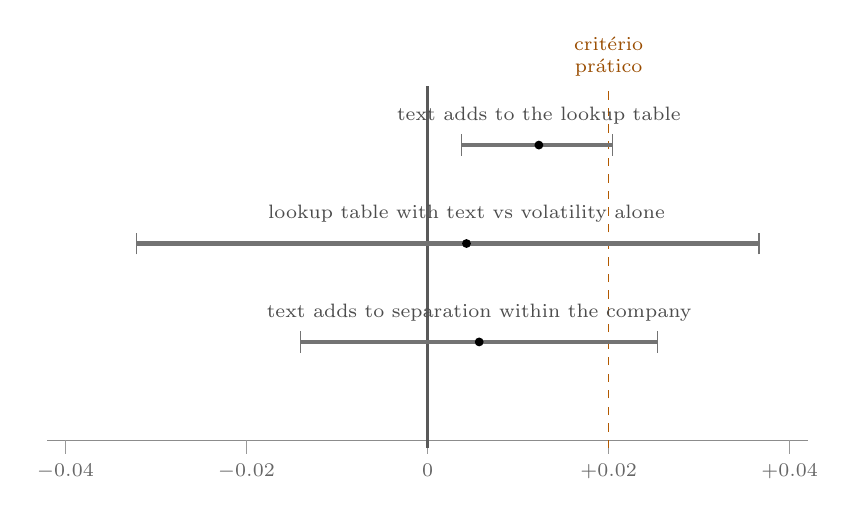
\begin{tikzpicture}[font=\small, x=115cm, y=1.25cm]
  \draw[black!45] (-0.042,0) -- (0.042,0);
  \foreach \xv/\xl in {-0.04/{$-0.04$}, -0.02/{$-0.02$}, 0/{$0$}, 0.02/{$+0.02$},
                       0.04/{$+0.04$}} {
    \draw[black!40] (\xv,0) -- (\xv,-0.14) node[below, font=\scriptsize, black!60] {\xl};
  }
  \draw[thick, black!65] (0,-0.08) -- (0,3.60);
  \draw[dashed, orange!70!black] (0.02,-0.08) -- (0.02,3.60)
    node[above, font=\scriptsize, text=orange!60!black, align=center] {critério\\ prático};

  \foreach \yv/\xa/\xm/\xb/\xrot in {
    3/0.0038/0.0123/0.0204/{text adds to the lookup table},
    2/-0.0321/0.0043/0.0366/{lookup table with text vs volatility alone},
    1/-0.0140/0.0057/0.0254/{text adds to separation within the company}} {
    \draw[line width=1.6pt, black!55] (\xa,\yv) -- (\xb,\yv);
    \draw[black!55] (\xa,\yv-0.11) -- (\xa,\yv+0.11);
    \draw[black!55] (\xb,\yv-0.11) -- (\xb,\yv+0.11);
    \fill[black] (\xm,\yv) circle (1.6pt);
    \node[above=4pt, font=\scriptsize, black!70, align=center] at (\xm,\yv) {\xrot};
  }
\end{tikzpicture}
\caption[Os três acréscimos, com intervalo de confiança]{Diferenças de desempenho e respetivos
intervalos de confiança a noventa e cinco por cento, obtidos por reamostragem por grupos. As duas
primeiras linhas são diferenças de \gls{PRAUC} e a terceira é uma diferença de capacidade de
ordenação dentro de cada empresa. Apenas a primeira exclui zero, e fá-lo abaixo do critério prático
fixado antes da medição.}
\label{fig:av_acrescimo}
\end{figure}

O título acrescenta a essa base $+0.012$ de \gls{PRAUC}, com intervalo entre $+0.004$ e
$+0.020$, que exclui zero. É a primeira ocasião em que uma representação de texto apresenta um
acréscimo detetável nesta tarefa, e o valor situa-se abaixo do critério prático de $0.02$ fixado
antes dos resultados.

Três reservas delimitam o alcance deste acréscimo, e todas são medições. A primeira é que a soma não
supera a volatilidade isolada: o valor obtido é de $0.547$ contra $0.542$, e a diferença tem
intervalo entre $-0.032$ e $+0.037$, que contém zero. A segunda é que o acréscimo não chega ao produto. A precisão dentro do orçamento de cinco alertas
por dia é de $0.662$ com e sem o texto, sem uma casa decimal de diferença. O acréscimo existe na
ordenação do conjunto completo e desaparece quando apenas cinco notícias por dia são selecionadas.

A terceira é que o texto
continua a não separar notícias da mesma empresa. A capacidade de ordenação dentro de cada empresa
vale $0.500$ por construção para a tabela de consulta e sobe para $0.512$ quando se lhe soma o
título. Para o modelo implantado é de $0.502$, com intervalo entre $0.462$ e $0.542$, e sobe
para $0.508$ com o texto, num acréscimo de $+0.006$ cujo intervalo, entre $-0.014$ e
$+0.025$, contém zero. Nenhum dos dois se distingue do acaso. A informação que o texto traz distingue empresas e períodos, e não
notícias.

A resposta à \gls{QI}3 mantém-se negativa e torna-se mais precisa. Nenhum modelo com texto supera a
volatilidade, e o texto não é inútil: acrescenta ao que o modelo já conhece sobre a empresa, de forma
pequena e mensurável. O que impede esse acréscimo de alterar o sistema não é a ausência de
informação, mas a natureza da informação, que distingue empresas quando o produto necessita de
distinguir notícias. O trabalho seguinte requer um rótulo por notícia, e não apenas um modelo de
maior dimensão.

Uma reserva final aplica-se ao próprio método. Este é mais um modelo avaliado sobre o mesmo bloco de
teste, que já serviu várias comparações do capítulo, e quanto mais vezes um conjunto de teste é
observado, mais provável se torna encontrar nele uma diferença pequena. As duas defesas utilizadas,
que consistem em não afinar a configuração e em declarar o critério antes da medição, reduzem esse
risco sem o eliminarem. A formulação que subsiste é a mais fraca das possíveis: não é possível
rejeitar que o título acrescente informação, e o acréscimo, a existir, é inferior ao critério prático
fixado antes da medição. Trata-se de um limite superior de um efeito e não de uma descoberta.

\subsection{Limites da conclusão}

O resultado não estabelece que o texto de notícias seja inútil. Foi avaliada uma única representação,
constituída por títulos sem o corpo do artigo, sobre um único corpus. Com textos completos e maior
volume de dados a resposta poderia ser distinta, o que constitui trabalho futuro.

Existe ainda uma hipótese alternativa que estas medições não excluem. O rótulo desconta o movimento
do mercado assumindo sensibilidade unitária, pela incoerência declarada na
Secção~\ref{sec:met_triagem}. Numa ação de sensibilidade elevada, o resíduo da subtração retém
movimento do mercado, pelo que o erro do rótulo não é aleatório: é maior nas ações mais sensíveis ao
mercado, que são tipicamente também as mais voláteis. Ora a linha de base vencedora é exatamente a
volatilidade. Com o que está medido não é possível separar a hipótese de a volatilidade prever melhor
a materialidade da hipótese de a volatilidade prever melhor o erro introduzido pelo rótulo. A experiência que resolveria a questão consiste em reconstruir o alvo com sensibilidades estimadas
e encolhidas, como faz a Secção~\ref{sec:met_decomposicao}, e repetir as seis famílias. Não foi
realizada. O nível e a ordenação das métricas ficam condicionados ao rótulo utilizado.

\section{O que permanece mensurável na decomposição}
\label{sec:av_decomposicao}

A decomposição do movimento não dá origem a uma questão de investigação. Esta secção estabelece a
razão dessa ausência e o que, apesar dela, permanece falsificável na técnica.

A diferença face às três técnicas anteriores é a existência de um alvo externo. Para a deteção existe
um critério de movimento extremo, o que permite contar acertos e falhas; para a recuperação existe
uma noção verificável de relevância, de que decorre a precisão@$k$; para a triagem existe um rótulo
construído a partir de preços posteriores. Em todos estes casos a técnica pode revelar-se errada
contra um alvo que lhe é exterior.

Na decomposição esse alvo não existe. Nenhuma fonte de dados publica qual foi a parcela verdadeira do
mercado no movimento de uma ação num dado dia, uma vez que essa quantidade não é observável e apenas
existe relativamente a um modelo. Fixadas as sensibilidades, a repartição é uma identidade
contabilística e não uma previsão suscetível de sair certa ou errada. A construção de uma medida de
exatidão neste ponto produziria um valor sem referente.

A técnica não fica por avaliar, mas por avaliar dessa forma, o que obriga a determinar o que nela
permanece falsificável. São duas propriedades, e ambas se medem sobre as dezassete empresas do mapa
de setores, que é o conjunto percorrido pelo procedimento de avaliação e não a lista monitorizada em
produção. A Figura~\ref{fig:av_motor} apresenta as duas.

\begin{figure}[ht]
\centering
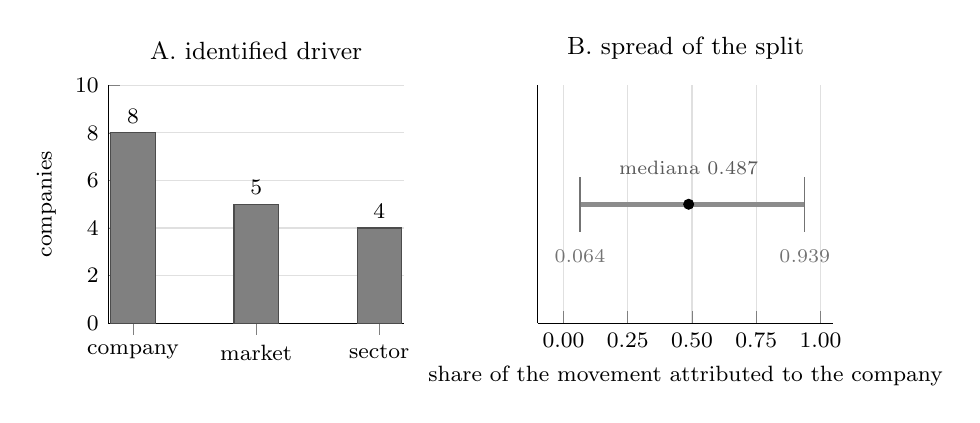
\begin{tikzpicture}
\begin{axis}[
  name=pa, width=0.44\textwidth, height=4.6cm, ybar, bar width=16pt,
  ymin=0, ymax=10, symbolic x coords={emp, merc, set}, xtick=data,
  xticklabels={company, market, sector}, ylabel={companies},
  nodes near coords, point meta=explicit symbolic,
  every node near coord/.append style={font=\footnotesize},
  title={\small A. identified driver},
  tick label style={font=\footnotesize}, label style={font=\footnotesize},
  ymajorgrids, grid style={black!12}, axis lines*=left,
]
\addplot[fill=black!50, draw=black!70] coordinates {(emp,8) [8] (merc,5) [5] (set,4) [4]};
\end{axis}
\begin{axis}[
  name=pb, at={(pa.right of origin)}, anchor=left of origin, xshift=1.7cm,
  width=0.44\textwidth, height=4.6cm,
  xmin=-0.10, xmax=1.05, ymin=0.4, ymax=1.6,
  ytick=\empty, xtick={0,0.25,0.5,0.75,1.0},
  xticklabels={{0.00},{0.25},{0.50},{0.75},{1.00}},
  xlabel={share of the movement attributed to the company},
  title={\small B. spread of the split},
  tick label style={font=\footnotesize}, label style={font=\footnotesize},
  xmajorgrids, grid style={black!12}, axis lines*=left,
]
\draw[line width=1.8pt, black!45] (axis cs:0.064,1) -- (axis cs:0.939,1);
\draw[black!55] (axis cs:0.064,0.86) -- (axis cs:0.064,1.14);
\draw[black!55] (axis cs:0.939,0.86) -- (axis cs:0.939,1.14);
\fill[black] (axis cs:0.487,1) circle (2pt);
\node[font=\scriptsize, black!65, anchor=south] at (axis cs:0.487,1.10) {mediana $0.487$};
\node[font=\scriptsize, black!55, anchor=north] at (axis cs:0.064,0.82) {$0.064$};
\node[font=\scriptsize, black!55, anchor=north] at (axis cs:0.939,0.82) {$0.939$};
\end{axis}
\end{tikzpicture}
\caption[A decomposição discrimina entre empresas no mesmo dia]{As dezassete empresas do mapa de
setores, decompostas no mesmo dia. Em A, a componente identificada como maior parcela do mesmo sinal
que o movimento observado. Em B, a dispersão da quota atribuída à empresa. A repartição produz
respostas distintas para empresas distintas no mesmo dia, que é a condição mínima para a sua
utilidade.}
\label{fig:av_motor}
\end{figure}

A primeira propriedade é a capacidade de discriminar. Uma decomposição que atribuísse a totalidade do
movimento à empresa em todos os dias seria inútil ainda que aritmeticamente correta. No dia medido, o
motor identificado foi a própria empresa em oito casos, o mercado em cinco e o setor em quatro, e a
quota do movimento atribuída à empresa apresentou mediana de $0.487$, com extremos em $0.064$ e
$0.939$.

A segunda propriedade é a qualidade da estimação das sensibilidades, e é a que pode efetivamente
estar errada. A medida apropriada é o coeficiente de determinação na janela de estimação, cuja
mediana foi de $0.460$. Não se trata do coeficiente do ajuste por mínimos quadrados, que, calculado
dentro da amostra e com termo constante, nunca poderia ser negativo, mas do coeficiente do modelo
efetivamente utilizado, com as sensibilidades já encolhidas e o termo constante recentrado. É esta a
medida adequada, por corresponder ao modelo cuja repartição é apresentada ao utilizador, e é por essa
razão que pode assumir valor negativo. Numa das dezassete empresas assumiu, o que significa que,
naquela janela, o mercado e o setor não explicavam a variação daquela ação melhor do que a sua própria
média, e que a repartição desse dia assenta num ajuste que não descreve os dados.

O resultado não estabelece que a repartição esteja correta pelo facto de as parcelas somarem. Elas
somam sempre, com diferença nula até à precisão da máquina, porque a parcela da empresa é definida
como resíduo, e uma repartição sem qualquer significado somaria igualmente. A soma exata constitui
uma verificação de implementação e não uma validação de método. O resultado também não estabelece que
o valor apresentado ao utilizador seja fiável em todos os dias, o que no caso de coeficiente negativo
não sucede, e é por essa razão que a limitação consta do Capítulo~\ref{cap:conclusoes}.

\section{O sistema em operação}
\label{sec:av_producao}

O quarto caso de estudo incide sobre o comportamento do sistema depois de implantado, sobre as
decisões que toma autonomamente. É a avaliação menos comum das três descritas na
Secção~\ref{sec:met_metodologia}, e a que produz o diagnóstico que alterou o sistema.

\subsection{O que a porta de decisão estava a separar}

A porta implantada era um limiar fixo sobre a probabilidade calibrada, que deixava passar as
candidatas acima de $0.50$. A pergunta com significado é a de saber se esse limiar separava títulos
ou separava empresas, e a medição foi realizada sobre as $4{,}366$ decisões efetivamente tomadas em
produção. A Figura~\ref{fig:av_porta} apresenta o resultado.

\begin{figure}[ht]
\centering
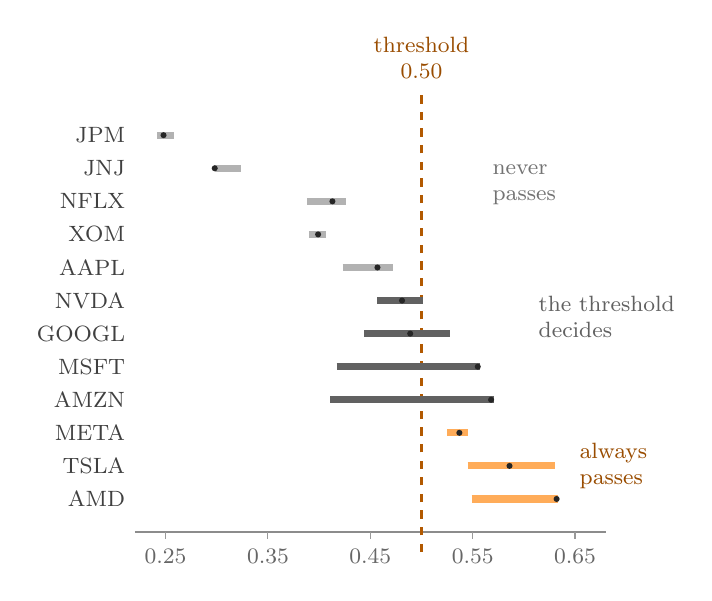
\begin{tikzpicture}[font=\footnotesize, x=13cm, y=0.42cm]
  \draw[black!45] (0.22,0) -- (0.68,0);
  \foreach \xv in {0.25,0.35,0.45,0.55,0.65}
    \draw[black!40] (\xv,0) -- (\xv,-0.22) node[below, black!60] {\xv};
  \draw[dashed, thick, orange!70!black] (0.50,-0.6) -- (0.50,13.4)
    node[above, align=center, text=orange!60!black] {threshold\\ $0.50$};
  \foreach \xn/\xtk/\xa/\xm/\xb/\xcor in {
    12/JPM/0.242/0.248/0.258/black!30, 11/JNJ/0.298/0.298/0.324/black!30,
    10/NFLX/0.388/0.413/0.426/black!30, 9/XOM/0.390/0.399/0.407/black!30,
    8/AAPL/0.423/0.457/0.472/black!30, 7/NVDA/0.457/0.481/0.501/black!62,
    6/GOOGL/0.444/0.489/0.528/black!62, 5/MSFT/0.417/0.555/0.557/black!62,
    4/AMZN/0.411/0.568/0.571/black!62, 3/META/0.525/0.537/0.545/orange!65,
    2/TSLA/0.545/0.586/0.630/orange!65, 1/AMD/0.549/0.632/0.633/orange!65}
  {
    \node[left, black!75] at (0.22,\xn) {\xtk};
    \draw[line width=2.6pt, color=\xcor] (\xa,\xn) -- (\xb,\xn);
    \fill[black!85] (\xm,\xn) circle (1.1pt);
  }
  \node[right, align=left, text=orange!60!black] at (0.645,2) {always\\ passes};
  \node[right, align=left, black!55] at (0.56,10.5) {never\\ passes};
  \node[right, align=left, black!62] at (0.605,6.5) {the threshold\\ decides};
\end{tikzpicture}
\caption[O que a porta de decisão separava]{Intervalo de todas as pontuações atribuídas pelo modelo a
cada empresa em produção, com a mediana assinalada. As barras claras nunca alcançam o limiar, as
escuras atravessam-no e as alaranjadas situam-se sempre acima. Oito das doze empresas encontram-se
inteiramente de um dos lados, o que significa que para essas a decisão estava tomada antes de o
título ser lido.}
\label{fig:av_porta}
\end{figure}

Os valores confirmam a leitura da figura. Sobre as $36{,}925$ decisões registadas, a amplitude média
das pontuações dentro de cada empresa é de $0.072$, ao passo que a amplitude entre as medianas das
empresas é de $0.392$, isto é, $5.4$ vezes superior. Duas empresas situavam-se sempre acima do
limiar e cinco nunca o alcançavam, pelo que apenas em cinco das doze o limiar chegava a decidir. Em $48\%$ dos títulos distintos o resultado estava determinado pela empresa antes de o título ser
lido. Contada por decisão registada, a fração sobe para $60\%$. Cita-se a primeira: a repontuação
dos mesmos títulos a cada ciclo de sessenta segundos inflaciona a segunda, e de forma desigual
entre empresas.

Numa janela anterior e mais curta, de $4{,}366$ decisões, os mesmos
indicadores valiam $0.064$, $0.385$ e $6.1$ vezes, com três empresas sempre acima e quatro em
que o limiar decidia. A conclusão estrutural não depende da janela. Em nenhuma das avaliações
registadas a Apple alcançou o limiar, com um máximo observado de $0.472$, ao passo que a AMD o
ultrapassou em todas.

As duas contagens medem quantidades distintas e ambas são reportadas. O sistema repontua os mesmos
títulos a cada ciclo de sessenta segundos, e a duplicação é maior nas empresas com menos notícias,
que são as que nunca ultrapassam o limiar, pelo que contar decisões desloca a fração para cima.
Contada uma vez por título distinto, sobre uma janela mais ampla de $36{,}925$ decisões, a fração é de
$48\%$. A conclusão estrutural não depende da contagem escolhida: continuam a existir empresas
inteiramente de um dos lados do limiar, e a amplitude entre empresas continua a ser várias vezes a
amplitude dentro de cada uma.

O defeito tem a mesma forma que o identificado na Secção~\ref{sec:av_qi1}, uma camada acima. Naquele
caso, um limiar fixo sobre o retorno mede a volatilidade da empresa em vez da raridade do dia; neste,
um limiar fixo sobre uma pontuação quase constante por empresa ordena empresas em vez de notícias.

Nenhum dos testes automáticos existentes o cobria. O modelo foi avaliado sobre a distribuição do
conjunto de treino e implantado atrás de dois filtros que a alteram, e cada componente cumpria o seu
contrato. O teste que o teria apanhado é o que este trabalho passou a executar: comparar a amplitude
das pontuações dentro de cada empresa com a amplitude entre empresas. O
que estava errado era uma suposição sobre a ligação entre eles, não enunciada em nenhum ponto.
Corresponde à classe de custo que \textcite{sculley2015debt} arrumam sob dependências de dados e
emaranhamento entre componentes, com o sintoma que os autores descrevem: o sistema continua a
produzir valores de aparência normal.

Existe uma segunda causa possível, que os registos não permitem separar da primeira. Uma das nove entradas é o retorno do próprio dia. No treino corresponde ao movimento completo do
dia da notícia. Em produção é calculado sobre a última barra diária disponível, que durante a
sessão é o fecho da véspera ou uma barra incompleta. As duas causas produzem o mesmo sintoma, e
o registo, à data desta medição, guardava a probabilidade e o resultado mas não o valor das
entradas no momento da pontuação, pelo que a sua separação exigiria registar essas entradas e
voltar a observar durante semanas.

Essa instrumentação foi construída e implantada em 4 de setembro de 2026, e o registo passou a
guardar, por decisão, o valor de cada uma das nove entradas, a data da última barra de preço
utilizada e a identidade do modelo que pontuou. Duas consequências decorrem dela e nenhuma é um
resultado. A primeira é que as decisões anteriores a essa data permanecem não reproduzíveis a
partir do registo, uma vez que recalcular hoje as entradas de um dia passado utilizaria uma série
de preços que já contém o que veio a seguir; as medições deste capítulo assentam nessas decisões
e não são afetadas pela alteração. A segunda é que a janela de observação necessária para separar
as duas causas começou nessa data, e o critério de aceitação de qualquer comparação futura foi
fixado antes de existir candidato, pela mesma razão que o Capítulo~\ref{cap:metodologia}
invoca para as restantes experiências. Nada se afirma aqui sobre o seu desfecho.

A correção aparente consistiria em substituir o limiar fixo por um limiar relativo a cada empresa. A simulação dessa alternativa sobre as mesmas decisões resolve metade do problema, uma vez que as
doze empresas passam a estar representadas, e introduz outro. Nas empresas cuja pontuação quase
não varia, o percentil recai sobre a constante e quase todas as decisões empatam acima dele; uma
delas passa a gerar $874$ alertas. O limiar relativo deixa de escolher por materialidade e passa a
escolher por desempate, que é precisamente o artefacto documentado na Secção~\ref{sec:av_qi3}. Dentro
de uma empresa a pontuação do modelo quase não varia com o título, e nenhuma regra de decisão
aplicada a essa pontuação a pode tornar sensível à notícia, porque a informação que distinguiria um
título do seguinte não está presente.

Em consequência, o modelo deixou de constituir porta e passou a constituir critério de ordenação, que
é a utilização que a medição sustenta, e o controlo de volume passou para um orçamento diário de
cinco alertas. Esta alteração aproxima duas políticas que divergiam: a dissertação avaliava uma
política de orçamento e o sistema implantava uma política de limiar, pelo que o valor reportado
descrevia um sistema distinto do que estava em funcionamento. As duas políticas passaram a pertencer
à mesma família sem se tornarem idênticas.

A alteração foi medida sobre os alertas efetivamente entregues, e o efeito pretendido
verifica-se. A quantidade observada é a concentração, definida como a fração dos alertas que
pertence às três empresas mais alertadas, e a sua vantagem é ser adimensional, o que permite
comparar janelas de dimensões distintas. Nos alertas de notícia, que são os que o orçamento
governa, a concentração desce de $0.713$ para $0.480$, com intervalo de confiança da
diferença a excluir zero, e o número de empresas que chegam a produzir um alerta passa de sete
para nove das doze monitorizadas.

O que sustenta a leitura não é, porém, a descida isolada, mas a comparação com uma série que a
alteração não governa. Os alertas de movimento de preço atravessam o mesmo período, as mesmas
empresas e as mesmas condições de mercado, e o orçamento diário não os conta. Nessa série a
concentração passa de $0.449$ para $0.485$, com o intervalo a conter zero. A quantidade
governada deslocou-se e a quantidade não governada não, o que afasta a explicação alternativa
de que o mercado se teria distribuído de forma mais uniforme no segundo período.

Cinco dias são excluídos da janela posterior, e a razão é registada por ser ela própria um
resultado. Entre 25 e 29 de agosto de 2026 o contador diário residia em disco efémero e
regressava ao valor inicial a cada arranque do processo, o que produziu séries de exatamente
cinco alertas nos instantes dos arranques e um dia com vinte. Nesses dias o orçamento não estava
em vigor, e a sua inclusão elevaria a concentração posterior para $0.514$. A reamostragem é
efetuada por dia, que é a unidade sobre a qual o orçamento atua.

A comparação não constitui um ensaio aleatorizado. A série de controlo partilha o período mas não
foi atribuída ao acaso, e as duas janelas diferem em duração e em condições de mercado. O que se
estabelece é que a quantidade governada se deslocou e a não governada não, e não que nenhuma
outra causa exista.

A métrica avaliada ordena todas as candidatas do bloco de
teste e apenas depois preenche cinco lugares em cada dia, o que exige conhecer o dia completo antes
de decidir e constitui por isso uma política diferida. O sistema implantado decide em linha, de
sessenta em sessenta segundos, e gasta o primeiro lugar na primeira notícia que atravesse as portas,
porque no momento da decisão a notícia da tarde ainda não existe. A precisão dentro do orçamento
reportada neste capítulo é, por conseguinte, um limite superior do que a política implantada obtém.

\subsection{O desempenho do modelo sobre as decisões que tomou}

O sistema regista todas as decisões de triagem e, decorridos os dias necessários para o preço
responder, confronta-as com o resultado efetivo. Duas medições resultam desse registo: a fração de
casos que se revelaram materiais de cada lado da porta, e a capacidade de ordenação do modelo,
medida pela \gls{ROCAUC}. A Figura~\ref{fig:av_posvalidacao} apresenta ambas, sobre $825$ decisões
já maturadas.

\begin{figure}[ht]
\centering
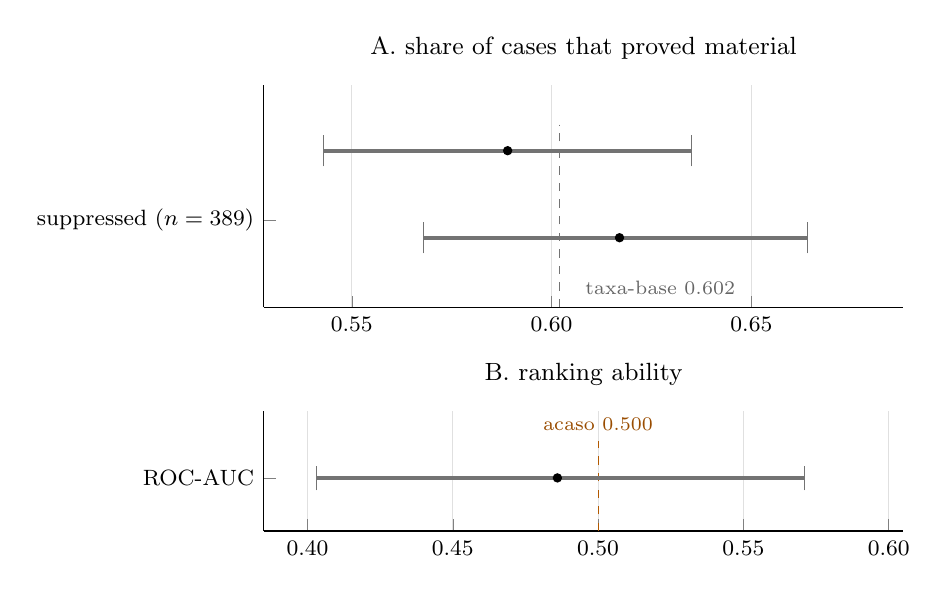
\begin{tikzpicture}
\begin{axis}[
  name=pa, width=0.80\textwidth, height=4.4cm,
  xmin=0.528, xmax=0.688, ymin=0.20, ymax=2.75,
  ytick={1.2}, yticklabels={{suppressed ($n = 389$)}, {kept ($n = 436$)}},
  xtick={0.55,0.60,0.65}, xticklabels={{0.55},{0.60},{0.65}},
  title={\small A. share of cases that proved material},
  tick label style={font=\footnotesize}, label style={font=\footnotesize},
  xmajorgrids, grid style={black!12}, axis lines*=left,
]
\addplot[draw=none, forget plot] coordinates {(0.60,1.5)};
\draw[dashed, black!55] (axis cs:0.602,0.20) -- (axis cs:0.602,2.30);
\node[font=\scriptsize, black!60, anchor=west] at (axis cs:0.606,0.42) {taxa-base $0.602$};
\draw[line width=1.4pt, black!55] (axis cs:0.543,2) -- (axis cs:0.635,2);
\draw[black!55] (axis cs:0.543,1.82) -- (axis cs:0.543,2.18);
\draw[black!55] (axis cs:0.635,1.82) -- (axis cs:0.635,2.18);
\fill[black] (axis cs:0.589,2) circle (1.7pt);
\draw[line width=1.4pt, black!55] (axis cs:0.568,1) -- (axis cs:0.664,1);
\draw[black!55] (axis cs:0.568,0.82) -- (axis cs:0.568,1.18);
\draw[black!55] (axis cs:0.664,0.82) -- (axis cs:0.664,1.18);
\fill[black] (axis cs:0.617,1) circle (1.7pt);
\end{axis}
\begin{axis}[
  name=pb, at={(pa.below south west)}, anchor=north west, yshift=-9mm,
  width=0.80\textwidth, height=3.1cm,
  xmin=0.385, xmax=0.605, ymin=0.4, ymax=1.75,
  ytick={1}, yticklabels={ROC-AUC},
  xtick={0.40,0.45,0.50,0.55,0.60},
  xticklabels={{0.40},{0.45},{0.50},{0.55},{0.60}},
  title={\small B. ranking ability},
  tick label style={font=\footnotesize}, label style={font=\footnotesize},
  xmajorgrids, grid style={black!12}, axis lines*=left,
]
\addplot[draw=none, forget plot] coordinates {(0.50,1)};
\draw[dashed, orange!70!black] (axis cs:0.50,0.4) -- (axis cs:0.50,1.42);
\node[font=\scriptsize, text=orange!60!black, anchor=south] at (axis cs:0.50,1.42)
  {acaso $0.500$};
\draw[line width=1.4pt, black!55] (axis cs:0.403,1) -- (axis cs:0.571,1);
\draw[black!55] (axis cs:0.403,0.86) -- (axis cs:0.403,1.14);
\draw[black!55] (axis cs:0.571,0.86) -- (axis cs:0.571,1.14);
\fill[black] (axis cs:0.486,1) circle (1.7pt);
\end{axis}
\end{tikzpicture}
\caption[O modelo sobre as decisões que tomou em produção]{Em A, a fração de casos que se revelaram
materiais entre as decisões que o modelo deixou passar e entre as que travou, com intervalos de
confiança a noventa e cinco por cento e a taxa-base do conjunto. As suprimidas apresentam fração
superior às mantidas, mas os dois intervalos sobrepõem-se em quase toda a extensão e não as
separam. Em B, a capacidade de ordenação medida sobre as $239$ unidades independentes, com o
intervalo a conter confortavelmente o valor de acaso.}
\label{fig:av_posvalidacao}
\end{figure}

Sobre a população que efetivamente observa, esta amostra não distingue o modelo do acaso em nenhuma
das duas medidas. As notícias que deixou passar revelaram-se materiais em $58.9\%$ dos casos,
contra $61.7\%$ das que travou, sobre uma taxa-base de $60.2\%$; os intervalos das duas frações
sobrepõem-se, pelo que a ordenação aparente não é estabelecida. O que fica medido é a ausência de
benefício detetável com esta dimensão de amostra, e não a ausência de benefício.

Estes valores exigem uma reserva de precisão considerável: as $825$ decisões
não constituem $825$ observações independentes, dado que o rótulo é atribuído por par formado pela
empresa e pelo dia, e as linhas repartem-se por apenas $239$ pares distintos. Medida sobre essas
unidades, a capacidade de ordenação situa-se em $0.486$ com intervalo de confiança entre $0.403$
e $0.571$, num intervalo em que o acaso vale exatamente $0.500$. A leitura correta não é a de que
o modelo seja pior do que a ausência de modelo, mas a de que esta amostra não o distingue do acaso.

A medição foi repetida quando o registo dispunha de $825$ decisões maturadas contra as $530$ da
primeira leitura, e quase nada se alterou: a diferença entre mantidas e suprimidas estreitou-se, a
capacidade de ordenação passou de $0.494$ para $0.486$ e o intervalo encolheu. Com metade mais
evidência, o veredicto mantém-se e torna-se mais firme.

A explicação mais provável não é a de que o modelo esteja avariado, mas a de que esteja em excesso.
Quando é invocado, as notícias já atravessaram o filtro de relevância e o filtro de frescura, e esses
filtros elementares removeram grande parte daquilo que o modelo foi treinado para remover, restando
pouco para separar. Um modelo avaliado isoladamente e implantado atrás de filtros nunca foi avaliado
na distribuição que efetivamente observa, e esta é a constatação com maior capacidade de
transferência do trabalho.

Três das doze empresas monitorizadas, a AMD, a Netflix e a Meta, não figuram no corpus de treino, e
uma quarta, a Microsoft, figura apenas no bloco de teste. O modelo pontua-as na mesma, porque o que
recebe são valores numéricos e não a identidade da empresa, mas fá-lo sobre uma combinação de
entradas que não observou. Duas das ausentes, a AMD e a Meta, estão entre as que se situam sempre
acima do limiar, pelo que a determinação por empresa descrita acima se concentra precisamente em
nomes que o modelo nunca observou. Constitui um segundo sentido, mais literal, em que o modelo
implantado opera fora da distribuição em que foi avaliado, e as decisões dessas empresas entram
nas $825$ acima como quaisquer outras.

\subsection{Deriva das distribuições}

Uma segunda razão, independente da anterior, pode fazer com que um modelo implantado deixe de servir:
os dados alteram-se. O modelo foi treinado sobre o período de 2018 a 2023 e opera em 2026. A medida
utilizada é o \gls{PSI}, que confronta aqui a distribuição de cada entrada no bloco de treino,
compreendido entre 2018 e 2022, com a do bloco de teste, de 2023. Não é, portanto, a distância entre
o treino e o presente, que a subsecção seguinte discute em separado: é a deriva interna ao próprio
protocolo. As bandas são as convencionadas em risco de crédito, segundo as quais valores
abaixo de $0.10$
indicam estabilidade, valores entre $0.10$ e $0.25$ deslocamento moderado e valores acima de
$0.25$ deslocamento significativo. A Figura~\ref{fig:av_deriva} apresenta o resultado.

\begin{figure}[ht]
\centering
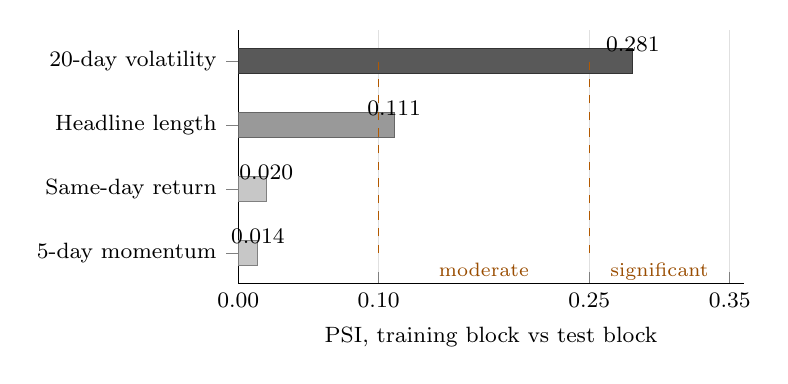
\begin{tikzpicture}
\begin{axis}[
  xbar, width=0.66\textwidth, height=4.8cm, bar width=9pt,
  xmin=0, xmax=0.36, enlarge y limits=0.16,
  symbolic y coords={mom, ret, comp, vol}, ytick={mom, ret, comp, vol},
  yticklabels={5-day momentum, Same-day return, Headline length,
               20-day volatility},
  nodes near coords, nodes near coords align={horizontal}, point meta=explicit symbolic,
  every node near coord/.append style={font=\footnotesize},
  xlabel={\gls{PSI}, training block vs test block},
  xtick={0,0.10,0.25,0.35}, xticklabels={{0.00},{0.10},{0.25},{0.35}},
  tick label style={font=\footnotesize}, label style={font=\footnotesize},
  xmajorgrids, grid style={black!12}, axis lines*=left,
]
\addplot[bar shift=0pt, fill=black!22, draw=black!50] coordinates {(0.014,mom) [0.014] (0.020,ret) [0.020]};
\addplot[bar shift=0pt, fill=black!40, draw=black!60] coordinates {(0.111,comp) [0.111]};
\addplot[bar shift=0pt, fill=black!65, draw=black!80] coordinates {(0.281,vol) [0.281]};
\draw[dashed, orange!70!black] (axis cs:0.10,mom) -- (axis cs:0.10,vol);
\draw[dashed, orange!70!black] (axis cs:0.25,mom) -- (axis cs:0.25,vol);
\node[font=\scriptsize, text=orange!60!black, anchor=north] at (axis cs:0.175,mom) {moderate};
\node[font=\scriptsize, text=orange!60!black, anchor=north] at (axis cs:0.30,mom)
  {significant};
\end{axis}
\end{tikzpicture}
\caption[Deslocamento das distribuições de entrada]{Índice de estabilidade populacional de cada
entrada entre o bloco de treino, de 2018 a 2022, e o bloco de teste, de 2023, com as bandas
convencionadas assinaladas. A entrada de que o modelo mais depende é a que mais se deslocou. A
prevalência do rótulo passa de $0.3854$ para $0.3781$ entre as duas pontas, mas não é estável
pelo meio: no bloco de validação, temporalmente entre ambas, chega a $0.4704$.}
\label{fig:av_deriva}
\end{figure}

O resultado tem duas metades. A entrada que mais se deslocou é a volatilidade dos vinte dias
anteriores, situada na banda significativa, ao passo que as restantes permanecem estáveis ou
moderadas. O rótulo desloca-se pouco entre as pontas, com a prevalência de positivos a passar de
$0.3854$ para $0.3781$, mas não é estável: o bloco de validação, temporalmente entre os dois,
chega a $0.4704$. A prevalência oscila com o regime de volatilidade em vez de derivar numa
direção, o que é coerente com a volatilidade ser a entrada que mais se desloca.

A leitura correta desta medição é a de que a deriva não é externa aos valores deste capítulo: é a
que o próprio protocolo atravessa, uma vez que treina em 2018--2022 e avalia em 2023. A \gls{PRAUC}
reportada é já uma medida sob esta deriva, e a combinação é desfavorável porque a entrada de que o
modelo mais depende é precisamente a que mais se deslocou.

O que esta medição não estabelece é a distância entre o treino e 2026, que é o período em que o
sistema opera. Um instantâneo sobre cotações atuais aponta na mesma direção, com a volatilidade a ser de novo a
entrada que mais se desloca. Assenta, porém, em janelas deslizantes consecutivas que partilham a
quase totalidade das observações, o que inflaciona o índice e torna a sua magnitude não comparável
com a da figura. O valor permanece por medir, e não é estimado por analogia. A
deriva é, em qualquer dos casos, medida e não corrigida, e a Secção~\ref{sec:con_futuro} enuncia o
que seria necessário para a corrigir.

\subsection{O sistema completo contra as alternativas existentes}

As secções anteriores comparam componente a componente. Falta a comparação ao nível do sistema:
dadas as notícias de um dia, a política escolhe as cinco a apresentar melhor do que uma regra
disponível sem custo. A Figura~\ref{fig:av_pontaaponta} responde. Todas as políticas escolhem cinco
por dia, sobre o mesmo bloco de teste e com o mesmo rótulo, e o desempate é aleatório e explícito em
todas.

\begin{figure}[ht]
\centering
\begin{tikzpicture}
\begin{axis}[
  ig axis, xbar, width=0.68\textwidth, height=5.4cm, bar width=10pt,
  xmin=0, xmax=1.12, enlarge y limits=0.14,
  symbolic y coords={acaso, mexeu, modelo, volat, oraculo},
  ytick={acaso, mexeu, modelo, volat, oraculo},
  yticklabels={Random choice, Biggest mover today, The deployed model,
               Company volatility, Oracle},
  nodes near coords, nodes near coords align={horizontal}, point meta=explicit symbolic,
  every node near coord/.append style={font=\footnotesize},
  xlabel={precision@5 under the same protocol},
  tick label style={font=\footnotesize}, label style={font=\footnotesize},
  xmajorgrids, grid style={black!12}, axis lines*=left,
]
\addplot[bar shift=0pt, ig reference bar] coordinates {(0.375,acaso) [0.375]};
\addplot[bar shift=0pt, ig alternative bar] coordinates {(0.489,mexeu) [0.489] (0.662,volat) [0.662]};
\addplot[bar shift=0pt, ig current bar] coordinates {(0.632,modelo) [0.632]};
\addplot[bar shift=0pt, ig reference bar] coordinates {(0.968,oraculo) [0.968]};
\end{axis}
\end{tikzpicture}
\caption[O sistema contra as alternativas já disponíveis]{Cinco políticas de seleção sobre o mesmo
bloco de teste. A escolha aleatória serve de referência; o oráculo é um máximo teórico não utilizável,
obtido com conhecimento das respostas. Todas escolhem conhecendo o dia
completo, pelo que cada valor é um limite superior do que a mesma regra obteria decidindo ao minuto.}
\label{fig:av_pontaaponta}
\end{figure}

Três leituras resultam da figura. A primeira é que o sistema supera a alternativa realista: apresentar
notícias das empresas com maior movimento do dia é o que qualquer aplicação de bolsa já faz sem
custo, e obtém $0.489$, contra $0.632$ do sistema, um ganho de $0.143$ sob o mesmo protocolo.
Este valor mede a capacidade de ordenar o rótulo aproximado no bloco histórico, e não a utilidade
percebida por uma pessoa nem o valor causal dos alertas em funcionamento.

A segunda é que o sistema continua a não superar a volatilidade. Treze constantes calculadas
exclusivamente sobre o bloco de treino obtêm $0.662$, o que é coerente com a ablação da
Secção~\ref{sec:av_ablacao}: o modelo é, na prática, uma tabela por empresa, e a volatilidade é outra
tabela por empresa, mais simples, sendo esta a que dispensa treino.

A terceira, e mais útil, é a localização da limitação pelo máximo teórico. O melhor resultado
possível, escolhendo com conhecimento das respostas, seria de $0.968$, o que significa que em quase
todos os dias existem efetivamente cinco notícias materiais no conjunto disponível. O sistema não
está limitado por escassez de matéria-prima, mas pela incapacidade de identificar quais são. A margem
entre $0.632$ e $0.968$ é de $0.336$ e reside quase integralmente na separação de notícias
dentro de cada empresa, que é precisamente o que o modelo implantado não consegue realizar. É a mesma
conclusão obtida por um terceiro caminho independente.

Todas as políticas desta comparação escolhem de entre o que a fonte entregou, o que deixa de fora a
pergunta anterior a todas, relativa aos dias em que nada foi entregue. Sobre um ano de notícias
captadas, existia pelo menos uma notícia relevante em $88.5\%$ dos dias que o detetor considerou
invulgares, num total de $417$, e em $47$ dos $52$ dias mais extremos, dimensão que não permite
distinguir as duas frações. Nos restantes, nenhuma alteração ao sistema produz
efeito, uma vez que uma notícia não associada à empresa pela fonte gratuita não chega a entrar no
percurso. A cobertura é ainda muito desigual, com a empresa pior coberta a situar-se nos $50\%$. Este
valor é um limite superior, e a distinção determina o que ele vale: estabelece que existia uma
notícia, e não que tenha chegado a notícia correta. A Secção~\ref{sec:con_limitacoes} retoma-o como
limitação.

Uma linha de base não foi medida, e a razão fica registada. A alternativa mais natural consistiria em
apresentar as primeiras cinco notícias a chegar. Não é mensurável neste protocolo, uma vez que o
conjunto de dados histórico não conserva a hora de publicação e está ordenado por data e por empresa,
pelo que utilizar a ordem do ficheiro mediria a ordem alfabética das empresas. Seria o mesmo
artefacto documentado na Secção~\ref{sec:av_qi3}, desta vez introduzido deliberadamente. Uma linha de
base errada é pior do que uma linha de base em falta.

% A subsecção da utilidade percebida é GERADA por scripts/analyse_feedback.py a partir dos
% votos recolhidos no canal, e não escrita à mão. É a mesma disciplina do resto do trabalho: o
% número aparece aqui porque veio do procedimento que o calculou. O ficheiro é correto com
% qualquer N — abaixo do mínimo pré-registado diz que não reporta proporção —, portanto a
% dissertação compila enquanto a recolha decorre e passa a estar certa quando ela fechar.
% GERADO por scripts/analyse_feedback.py — NÃO EDITAR À MÃO.
% Correr o script outra vez depois de a recolha fechar; o texto acompanha os dados.
\subsection{Perceived usefulness of the alerts delivered}
\label{sec:av_feedback}

The channel now accompanies every alert delivered with two buttons, \emph{useful} and \emph{did not help}, and records the vote of whoever presses. The analysis rules were fixed before a single vote existed and were not changed afterwards: a minimum of twenty effective votes to report any proportion, one vote per person and per alert with the last replacing the previous one, a safeguard that repeats the computation without the dominant voter when that voter accounts for more than forty per cent of the votes, always subject to the same minimum, and Wilson confidence intervals, calculated without adjustment for clustering.
Only votes on alerts present in the shared log were counted.

131 valid votes were recorded between 2026-09-02 and 2026-09-11, corresponding to 91 effective votes from 3 distinct people, on 62 alerts. 11 votes were later changed by the same person, and only the last of each pair counts. Another 29 repeat an earlier vote without changing it and count only once. A further 5 votes, not counted among the 131 above, were excluded for not corresponding to any alert in the shared log.

Of the 91 effective votes, 86 rated the alert as useful, that is 95\%, with a 95\% Wilson confidence interval between 88\% and 98\%. This binomial calculation does not adjust for dependence between votes by the same person or on the same alert; its width does not represent all the uncertainty in this sample.

A single person accounts for 58\% of the effective votes, above the limit of 40\% fixed in the protocol. Excluding that person, 38 votes remain, of which 34 rate the alert as useful.
The proportion without that person is 89\%, with an interval between 76\% and 96\%. This is the reading to retain.

The independence between whoever builds the system and whoever rates it is a condition of this sample: the author is not among the votes counted. The votes come from readers of the public channel, and the log keeps of each only the conversation identifier assigned by the platform.

These votes are observational feedback in a real context and do not replace the controlled study that Section~\ref{sec:con_limitacoes} identifies as the gap of greatest weight in this work, and which remains to be carried out.

Four limitations accompany this result and none of them is resolved by more votes. The first is self-selection: whoever wants to votes, and those who find an alert indifferent tend to press nothing, which pushes the sample towards the extremes. The second is the absence of a counterfactual, since no group received the price change without the explanation that accompanies it; nothing here attributes the usefulness to the explanation itself. The third is the distance between perceived usefulness and a better decision, which is the founding hypothesis of this work and remains untested. The fourth is not knowing who votes: the channel is public and it is not known whether those who answer belong to the audience the dissertation assumes.


\section{Síntese dos resultados}
\label{sec:av_sintese}

Esta secção reúne as comparações realizadas ao longo do trabalho, incluindo aquelas em que o sistema
mantém a opção que a medição não favorece.

Duas das três respostas são afirmativas e uma é negativa. A resposta negativa é a que exigiu maior
esforço de verificação, e é também a que estabelece que a avaliação foi construída de modo a poder
produzir uma resposta negativa. A Tabela~\ref{tab:av_alternativas} apresenta cada escolha técnica ao
lado da alternativa medida contra ela.

\begin{table}[!htbp]
\caption[Cada escolha, contra a alternativa que não ficou]{As decisões técnicas do trabalho, cada uma
com a alternativa medida contra ela. Três linhas registam que a opção implantada não obteve o melhor
resultado, e a razão da sua manutenção consta da coluna respetiva. As três últimas linhas são
restrições fixadas antes de qualquer medição, e não resultados: apresentá-las como comparação
atribuir-lhes-ia uma autoridade que não possuem.}
\label{tab:av_alternativas}
\centering
\scriptsize
\begin{tabular}{L{0.19\textwidth} L{0.30\textwidth} L{0.39\textwidth}}
\toprule
\tabhead{Opção implantada} & \tabhead{Alternativa medida} & \tabhead{Leitura} \\
\midrule
\emph{z}-score deslizante & Limiar fixo de três por cento: amplitude $0.344$ contra $0.015$ &
Um limiar fixo mede a volatilidade da empresa e não a raridade do dia. \\
\addlinespace
\emph{z}-score deslizante & \emph{Isolation Forest} com $F_1$ de $0.269$ e \emph{Local Outlier
Factor} com $0.280$, contra $0.530$ & Os detetores aprendidos assinalam quase tudo e acertam
pouco. \\
\addlinespace
Janela de vinte dias & Não obteve o melhor resultado: dez dias produzem $F_1$ de $0.385$, vinte
dias $0.516$ e sessenta dias $0.678$ & A medição favorece a janela mais longa. Mantida por
responsividade, com a reserva de circularidade do rótulo declarada. \\
\addlinespace
Desvio-padrão de pesos iguais & Não obteve o melhor resultado: o decaimento exponencial produz $F_1$
de $0.664$ contra $0.516$ & Mantido por ser explicável a um leitor não especializado, e
registado como escolha e não como resultado. \\
\addlinespace
Embeddings de frase & Sobreposição de palavras: precisão@5 de $0.346$ contra $0.514$ &
Vocabulário comum não implica assunto comum, e assunto comum não exige vocabulário comum. \\
\addlinespace
MiniLM em vez de MPNet & Não obteve o melhor resultado: o MPNet produz $0.538$ contra $0.514$; um
codificador de domínio financeiro produz $0.420$ & O modelo mais pesado é melhor e foi substituído
por custo. O codificador de domínio obteve o pior resultado de todos, por medição e não por
suposição. \\
\addlinespace
Regressão logística & Árvores com reforço do gradiente: \gls{PRAUC} de $0.469$ contra $0.538$ &
O modelo mais expressivo não obteve melhor resultado, e o modelo simples é explicável. \\
\addlinespace
Calibração de Platt & Regressão isotónica, comparada sobre a mesma validação & A calibração de Platt
iguala ou supera no índice de Brier em todas as famílias avaliadas. \\
\addlinespace
Semelhança do cosseno & Distância euclidiana & Com vetores normalizados as duas produzem a mesma
ordenação, e a primeira dispõe de leitura mais direta. \\
\addlinespace
Dois gatilhos, notícia e preço & Fusão com o volume e a intensidade de notícia, na linha dos painéis
que combinam sinais de origens distintas \autocite{worldmonitor2026}: perde em dois dos três
orçamentos, com $-0.050$ e $-0.032$, e ganha no terceiro por $+0.004$ & Um ganho que depende do
orçamento escolhido, e uma ordem de grandeza menor do que as perdas, não sustenta a adoção. O volume
continua a ser calculado e apresentado como contexto, sem originar alertas. \\
\midrule
Apenas fontes gratuitas & --- & Restrição fundadora: define o público que o sistema pode servir. \\
Ausência de previsão de preços & --- & Restrição de desenho: é o que torna verificável tudo o
restante. \\
Mercado dos Estados Unidos & --- & Restrição de âmbito: é onde as fontes gratuitas apresentam
cobertura. \\
\bottomrule
\end{tabular}
\end{table}

Três linhas da tabela merecem desenvolvimento. A primeira respeita ao codificador de domínio
financeiro, cuja derrota tem explicação no objetivo de treino e não no conhecimento do domínio,
conforme a Secção~\ref{sec:av_qi2} estabelece. A segunda respeita à janela de vinte dias, que é a
opção mais difícil de justificar, uma vez que a única medição existente sobre este ponto não a
sustenta e a justificação de responsividade não é quantitativa. A terceira respeita ao estimador de
volatilidade, mantido por explicabilidade contra uma alternativa medida como superior.

O capítulo documenta três ocasiões em que uma técnica mais simples superou uma técnica mais
sofisticada em condições equivalentes, e três ocasiões em que sucedeu o inverso e o sistema
conservou mesmo assim a opção implantada. Nestas últimas a razão difere em cada caso, e nenhuma
delas é o resultado da medição: o estimador de pesos iguais foi mantido por explicabilidade, a
janela de vinte dias por responsividade, e o codificador de frases mais pequeno por custo
computacional. A distinção entre os dois conjuntos é a distinção entre resultado e escolha, e o
Capítulo~\ref{cap:conclusoes} retoma-a ao estabelecer o que este trabalho demonstra e o
que apenas decide.
